% ============================================================
\section{Analyse Empirique des Données ADEME : Résultats et Interprétation}
% ============================================================

Dans la continuité de la revue de littérature soulignant la nécessité de dépasser les biais de confusion liés aux caractéristiques physiques des véhicules, cette section présente les résultats de notre modélisation empirique fondée sur les données de certification de l'ADEME. L'objectif central de cette démarche est de déconstruire la « vision tunnel » focalisée exclusivement sur le CO2, en intégrant à l'analyse les polluants locaux à impact sanitaire immédiat, tels que les oxydes d'azote (NOx) et les hydrocarbures imbrûlés (HC).

Cependant, comparer directement les niveaux d'émissions bruts entre différents modèles de véhicules expose l'analyse à un biais de confusion majeur : un véhicule lourd et puissant émettra mécaniquement davantage de polluants, masquant ainsi l'efficacité réelle de ses choix technologiques ou de ses systèmes de post-traitement. Pour neutraliser ce biais et isoler le « signal technologique » du « bruit physique », notre stratégie empirique se déploie en deux temps :

\par\vspace{0.9em}

\begin{itemize}
    \item[-] Une modélisation par Moindres Carrés Ordinaires (OLS) : Nous estimons d'abord des régressions linéaires multiples en logarithmes pour chaque polluant (CO2, HC, NOx). Ces modèles intègrent comme variables de contrôle les déterminants physiques incontournables identifiés dans la littérature, à savoir la masse, la puissance et le type de carrosserie. L'extraction des résidus de ces régressions nous permet d'isoler l'efficacité technologique "pure" des véhicules et d'étudier les éventuels compromis (trade-offs) entre les différents polluants.

    \vspace{0.5em}

    \item[-] Une analyse de Frontières Stochastiques (SFA) : Dans un second temps, nous dépassons l'approche par la moyenne (OLS) pour évaluer la performance individuelle de chaque véhicule par rapport à une frontière technologique optimale, mettant ainsi en lumière les disparités d'ingénierie au sein d'une même catégorie de motorisation.
\end{itemize}

\subsection{Déterminants des émissions de CO2 : Une confirmation empirique de l'impact massique}

\begin{figure}[H]
    \centering
    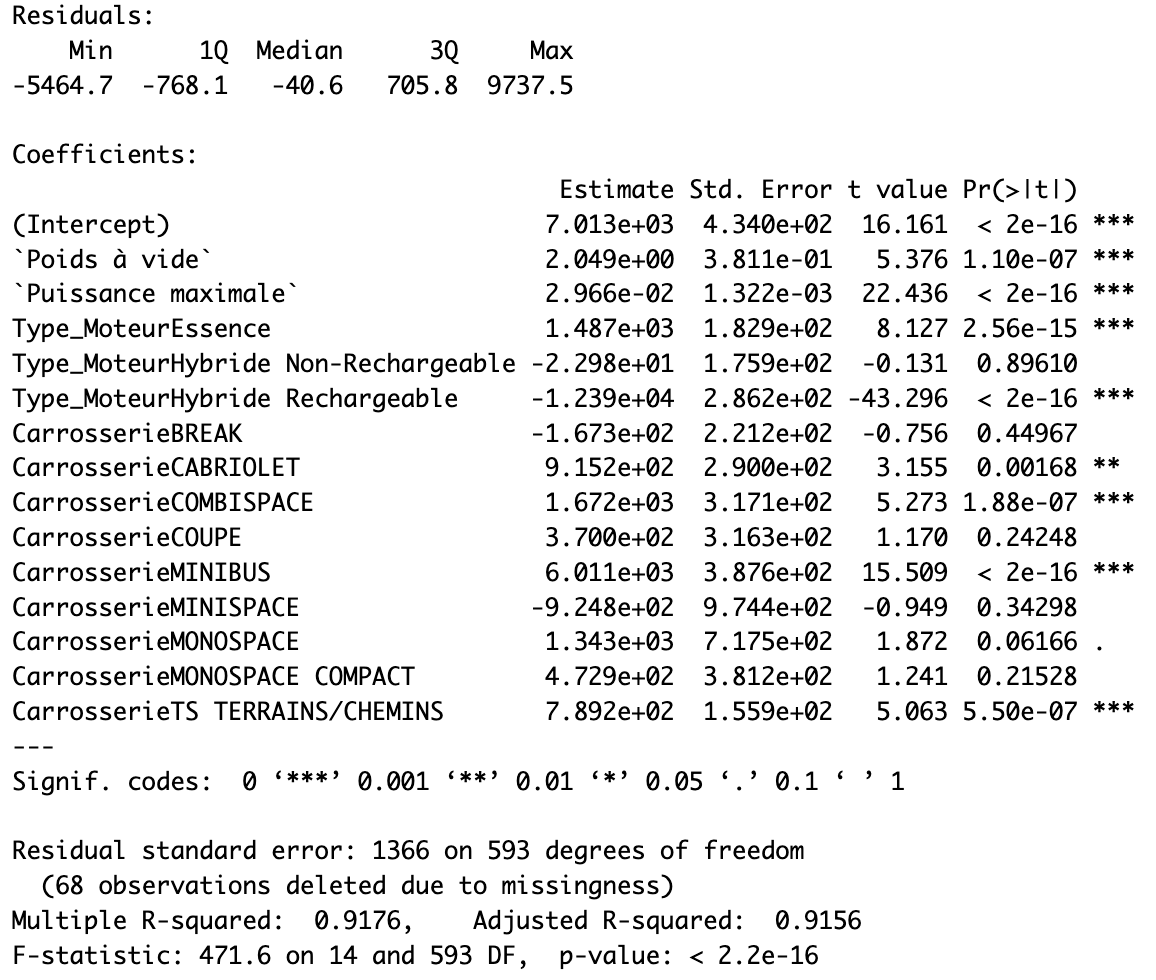
\includegraphics[width=0.78\textwidth]{résultats/OLS_CO2.png}
    \caption{Modèle OLS des émissions de CO2 : effets de la masse, de la puissance, de la motorisation et de la carrosserie.}
    \label{fig:ols_co2}
\end{figure}

Afin de quantifier l'impact des caractéristiques physiques et technologiques sur les émissions de dioxyde de carbone, nous avons estimé un modèle de régression linéaire multiple par la méthode des Moindres Carrés Ordinaires (OLS). La variable dépendante (CO2 mixte) est expliquée par la masse à vide, la puissance maximale, la motorisation (variable catégorielle) et le type de carrosserie.

\vspace{0.6em}

Qualité d'ajustement du modèle : Le modèle présente un pouvoir explicatif exceptionnellement élevé, avec un R2 ajusté de 0.9176. Cela signifie que près de 91,7 \% de la variance des émissions de CO2 homologuées est expliquée par ces seules variables structurelles. La statistique de Fisher globale (F-statistic = 471.6, p<2.2e-16) confirme la très forte significativité conjointe du modèle.

\vspace{0.6em}

Le poids et la puissance : des déterminants incompressibles :\\
Les résultats empiriques confirment sans ambiguïté les postulats de la physique fondamentale exposés précédemment :

\vspace{0.6em}

\begin{itemize}
    \item La masse à vide exerce un effet positif et hautement significatif (p<0.001). Indépendamment de la motorisation ou de l'aérodynamisme, l'augmentation du poids se traduit par une hausse mécanique des rejets de CO2, validant la relation directe avec l'énergie cinétique et les forces dissipatives (résistance au roulement).

    \vspace{0.5em}

    \item La puissance maximale présente également un coefficient positif et très fortement significatif (t=22.436), confirmant que le surdimensionnement des groupes motopropulseurs s'accompagne d'une pénalité environnementale incompressible. L'effet de la motorisation et l'artefact de l'hybride rechargeable : en prenant la motorisation Diesel comme modalité de référence (baseline implicite), l'analyse des coefficients met en exergue des dynamiques technologiques contrastées :

    \vspace{0.5em}

    \item Les véhicules à Essence présentent une pénalité significative (+1487 unités, p<0.001) par rapport au Diesel. Ce résultat est cohérent avec le meilleur rendement thermique historique des moteurs à allumage par compression (Diesel) face à l'allumage commandé (Essence).

    \vspace{0.5em}

    \item L'Hybride Non-Rechargeable ne présente pas de différence statistiquement significative avec la motorisation de référence (p=0.896).

    \vspace{0.5em}

    \item L'Hybride Rechargeable, en revanche, affiche un coefficient négatif massif et hautement significatif (-12390 unités). Loin d'être le seul reflet d'une efficience technologique, ce résultat empirique illustre parfaitement le biais du cycle d'homologation décrit dans la revue de littérature. Les tests WLTP, réalisés en grande partie sur l'autonomie de la batterie, écrasent artificiellement les émissions déclarées de ces véhicules, créant un artefact statistique majeur.

    \vspace{0.5em}

    \item L'impact de la carrosserie : le coût de la traînée aérodynamique. L'intégration du type de carrosserie permet de capturer, en partie, l'effet de la forme et de la surface frontale (S) sur la traînée aérodynamique. En prenant la berline classique comme référence probable, on observe que des formats volumineux comme les "MINIBUS" (+6011), les "COMBISPACE" (+1672) ou les "TS TERRAINS/CHEMINS" (catégorie incluant les SUV, +789.2) subissent tous des pénalités fortement significatives (p<0.001). Ces résultats démontrent que la mode des véhicules hauts et massifs annule une part substantielle des efforts d'optimisation réalisés sur les moteurs.
\end{itemize}

\subsection{Modélisation des émissions d'Hydrocarbures (HC) : La prédominance de la chimie sur la physique}

\begin{figure}[H]
    \centering
    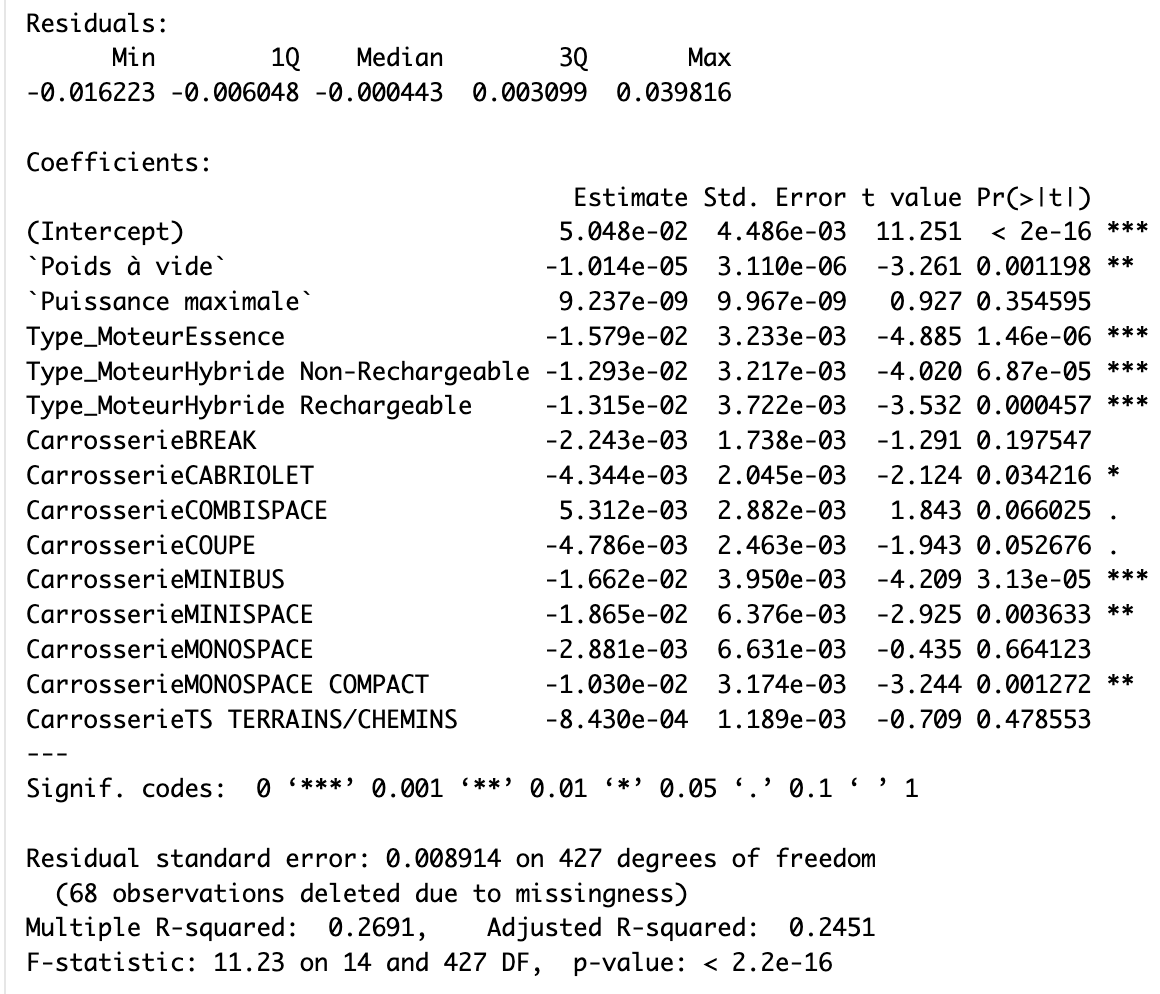
\includegraphics[width=0.78\textwidth]{résultats/OLS_HC.png}
    \caption{Modèle OLS des émissions d'hydrocarbures imbrûlés (HC).}
    \label{fig:ols_hc}
\end{figure}

Dans cette seconde étape, nous appliquons la même spécification économétrique aux émissions d'hydrocarbures imbrûlés (HC). Contrairement au CO2, qui est le produit naturel d'une combustion parfaite, les HC résultent d'une combustion incomplète. L'analyse des coefficients révèle une dynamique radicalement différente, soulignant le rôle crucial des systèmes de post-traitement.

\vspace{0.6em}

Le premier constat majeur réside dans la chute du coefficient de détermination. Le R2 ajusté s'établit ici à 0.2691. Seuls 26,9 \% de la variance des rejets de HC sont expliqués par les caractéristiques physiques du véhicule (poids, puissance, carrosserie). Ce résultat est théoriquement cohérent : contrairement au CO2, les émissions de HC ne sont pas dictées par les lois de l'énergie cinétique ou la masse à déplacer, mais par l'efficacité du pot catalytique, en particulier lors de sa phase de montée en température (démarrage à froid).

\vspace{0.6em}

L'analyse de la variable "Poids à vide" révèle un résultat empirique contre-intuitif mais fondamental : son coefficient est négatif (-1.014e-05) et statistiquement significatif (p < 0.01). En d'autres termes, plus un véhicule est lourd, moins il tend à émettre d'hydrocarbures imbrûlés. Ce phénomène s'explique par la thermodynamique du post-traitement : les véhicules plus lourds sont généralement équipés de moteurs de plus forte cylindrée qui dégagent davantage de chaleur. Cette inertie thermique supérieure permet au pot catalytique d'atteindre plus rapidement sa température optimale de fonctionnement lors des tests d'homologation, détruisant ainsi les HC plus précocement qu'un petit moteur peinant à chauffer son système d'échappement. À l'inverse, la variable "Puissance maximale" est statistiquement non significative (p = 0.354), confirmant qu'une fois le véhicule en mouvement, la puissance brute n'influence plus le traitement de ces imbrûlés.

\vspace{0.6em}

En conservant implicitement le Diesel comme modalité de référence, le modèle met en évidence la supériorité absolue des technologies à allumage commandé (Essence et Hybrides) dans le traitement spécifique des HC. Les coefficients des variables "Type\_MoteurEssence" (-1.579e-02), "Hybride Non-Rechargeable" (-1.293e-02) et "Hybride Rechargeable" (-1.315e-02) sont tous fortement négatifs et hautement significatifs (p < 0.001). Cela traduit l'efficacité redoutable et universelle du pot catalytique "3 voies" qui équipe ces motorisations. Comme évoqué dans notre revue de la chimie du moteur, l'oxydation des HC est une réaction robuste que l'industrie maîtrise aujourd'hui à la quasi-perfection, rendant ces motorisations intrinsèquement plus performantes sur ce polluant précis par rapport à la base de référence.

\vspace{0.6em}

Enfin, bien que certaines carrosseries affichent des coefficients significatifs (notamment les formats de type MINIBUS ou MINISPACE), leur influence reste secondaire par rapport à l'effet de la technologie de motorisation. L'hétérogénéité des rejets de HC se joue non pas sur l'aérodynamisme, mais dans le pot d'échappement.

\subsection{Modélisation des émissions d'Oxydes d'Azote (NOx) : L'empreinte du Diesel et le coût du post-traitement}

\begin{figure}[H]
    \centering
    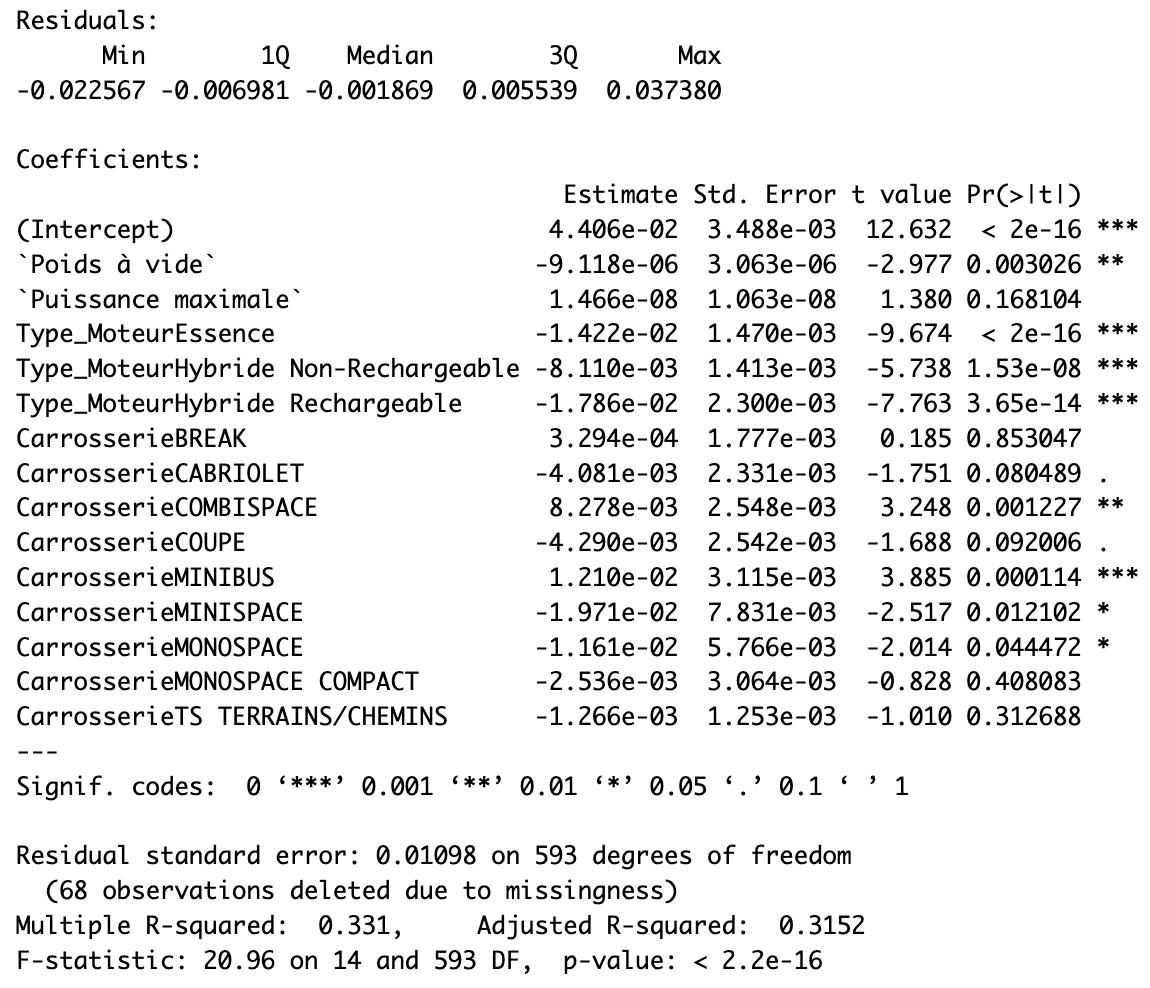
\includegraphics[width=0.78\textwidth]{résultats/OLS_Nox.png}
    \caption{Modèle OLS des émissions de NOx.}
    \label{fig:ols_nox}
\end{figure}

La troisième étape de notre démarche empirique s'attaque aux oxydes d'azote (NOx), un polluant sanitaire critique dont la formation répond à des lois thermodynamiques bien spécifiques. L'estimation OLS met en lumière la fracture technologique majeure qui sépare les différentes motorisations face à ce défi chimique. Le modèle affiche un R2 ajusté de 0.331. Ce score, bien qu'inférieur à celui du CO2, est supérieur à celui des HC. L'interprétation est claire : si les émissions de CO2 sont une fatalité physique (très bien expliquées par le poids et la puissance) et les HC un problème largement résolu par le catalyseur au démarrage, les émissions de NOx dépendent d'un compromis complexe entre la charge moteur et la sophistication du système de dépollution embarqué.

\vspace{0.6em}

Le résultat le plus spectaculaire de cette régression réside dans les coefficients des motorisations. En prenant le Diesel comme modalité de référence, on observe que les variables Type\_MoteurEssence (-1.422e-02), Hybride Non-Rechargeable (-8.110e-03) et Hybride Rechargeable (-1.786e-02) affichent toutes des coefficients négatifs massifs et statistiquement très significatifs (p<0.001). Ce résultat empirique valide de manière éclatante la théorie exposée dans notre première partie : les moteurs Diesel, fonctionnant intrinsèquement en mélange pauvre (excès d'air) et à des taux de compression très élevés, génèrent des températures internes favorisant massivement la réaction de Zeldovich. À l'inverse, les motorisations à allumage commandé (Essence et Hybrides) parviennent à contenir naturellement ces émissions ou à les traiter beaucoup plus efficacement grâce au pot catalytique 3 voies.

\vspace{0.6em}

L'analyse de la variable Poids à vide révèle un paradoxe apparent très instructif. Le coefficient est négatif (-9.118e-06) et significatif (p=0.003). Théoriquement, comme souligné dans la section 6.1, plus on cherche de la puissance pour compenser la masse, plus on crée des NOx toxiques à la source. Cependant, nos données mesurent les émissions à l'échappement (tailpipe), c'est-à-dire après le post-traitement. Ce coefficient négatif traduit une réalité industrielle et économique : les véhicules lourds, souvent plus onéreux et appartenant à des segments supérieurs, disposent de marges bénéficiaires suffisantes pour intégrer des systèmes de dépollution complexes et coûteux. Concrètement, un SUV lourd diesel sera systématiquement équipé d'un imposant système SCR (Selective Catalytic Reduction) avec injection d'AdBlue très performant, tandis qu'un véhicule léger et moins cher devra parfois se contenter d'un piège à NOx (LNT) moins efficace lors des variations de charge.

\vspace{0.6em}

Enfin, certaines carrosseries utilitaires ou volumineuses (MINIBUS, COMBISPACE) affichent des coefficients positifs et significatifs. Contrairement aux véhicules de tourisme haut de gamme, ces formats subissent souvent des cycles d'homologation où leur aérodynamisme défavorable force le moteur à opérer dans des plages de charge génératrices de NOx, sans toujours bénéficier des dispositifs de post-traitement les plus avancés.

\vspace{0.6em}

Ces régressions OLS démontrent que l'approche par la moyenne atteint ses limites : elle mélange les effets physiques purs (masse, aérodynamisme) avec les choix technologiques des constructeurs (budgets alloués au post-traitement). Pour évaluer véritablement l'efficience de ces choix d'ingénierie, il est désormais nécessaire d'analyser les résidus de ces modèles et de mesurer l'écart de chaque véhicule par rapport à la "frontière technologique" optimale via la méthode SFA.

\subsection{Analyse de Frontière Stochastique (SFA) : Mesure de l'efficience technologique}

Pour affiner notre compréhension des dynamiques d'émissions, nous avons complété l'approche par la moyenne (OLS) par une Analyse de Frontière Stochastique (SFA). Contrairement à l'estimation par les moindres carrés, la SFA permet d'estimer une "frontière" d'émissions optimales (minimales) compte tenu des contraintes physiques du véhicule (masse, puissance, carrosserie), et de mesurer l'écart spécifique de chaque modèle par rapport à cet optimum théorique.

\vspace{0.6em}

Afin de garantir la robustesse et la pertinence économique de nos résultats, nous avons fait le choix méthodologique d'estimer des modèles SFA distincts et indépendants pour chaque couple polluant/motorisation. La spécification économétrique retenue pour le terme d'inefficacité technique repose sur les paramétrages standards de la littérature, à savoir une distribution demi-normale (half-normal distribution). L'analyse qui suit s'appuie sur les graphiques de distribution de l'efficacité technique issus de ces modèles. Il est fondamental de préciser que cette efficacité est mesurée sur une échelle strictement comprise entre 0 et 1 : un score de 1 désigne un véhicule atteignant la perfection technologique (situé exactement sur la frontière de dépollution ou d'optimisation maximale), tandis qu'un score se rapprochant de 0 indique une inefficacité majeure par rapport aux capacités technologiques du marché.

\subsubsection{Efficacité technique CO2 des motorisations Essence : La preuve de la maturité technologique}

\begin{figure}[H]
    \centering
    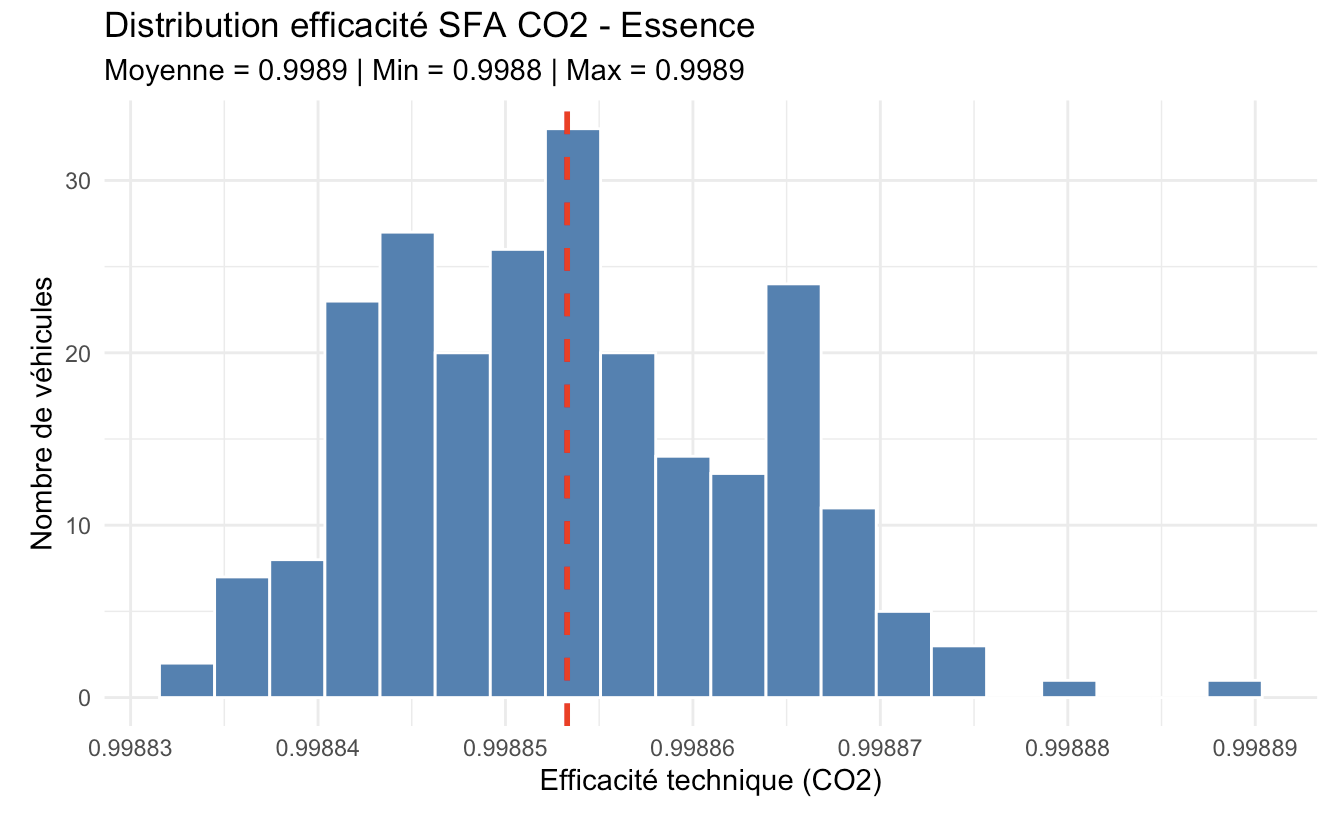
\includegraphics[width=0.74\textwidth]{résultats/SFA_CO2_Essence.png}
    \caption{Distribution SFA de l'efficacité CO2 -- motorisation Essence.}
    \label{fig:sfa_co2_essence}
\end{figure}

Le premier résultat issu de nos modèles SFA concerne la distribution de l'efficacité technique relative au CO2 pour le sous-échantillon des véhicules à motorisation Essence. Visuellement, l'histogramme généré par le modèle présente une distribution en cloche qui suggère de prime abord l'existence de disparités entre les véhicules. Toutefois, une analyse rigoureuse de l'échelle de l'axe des abscisses (efficacité technique, devant théoriquement s'étendre de 0 à 1) révèle une réalité radicalement différente : la variance de l'échantillon est en fait microscopique. L'intégralité des scores d'efficacité est compressée dans un intervalle infime, allant d'un minimum de 0.9988 à un maximum de 0.9989.

\vspace{0.6em}

Interprétation technologique : Ce resserrement extrême autour d'une efficacité relative quasi parfaite (score de 1) démontre que la technologie des moteurs thermiques purs à allumage commandé a atteint un plafond de maturité absolu concernant l'optimisation du rendement énergétique et, par extension, du CO2. En d'autres termes, à masse, puissance et carrosserie équivalentes, l'ingénierie de l'ensemble des constructeurs automobiles converge vers la même frontière technologique maximale permise par la thermodynamique.

\vspace{0.6em}

Ce résultat SFA corrobore de manière éclatante nos conclusions précédentes : la marge de manœuvre technologique pour améliorer le moteur thermique essence pur est aujourd'hui virtuellement nulle. Les disparités d'émissions brutes de CO2 observées sur les routes ne s'expliquent plus par l'efficience du moteur d'un constructeur par rapport à un autre, mais sont intégralement dictées par les déterminants physiques incompressibles, à savoir la masse à mettre en mouvement et l'aérodynamisme du véhicule.

\subsubsection{Efficacité technique CO2 des motorisations Diesel : Un diagnostic de saturation technologique identique}

\begin{figure}[H]
    \centering
    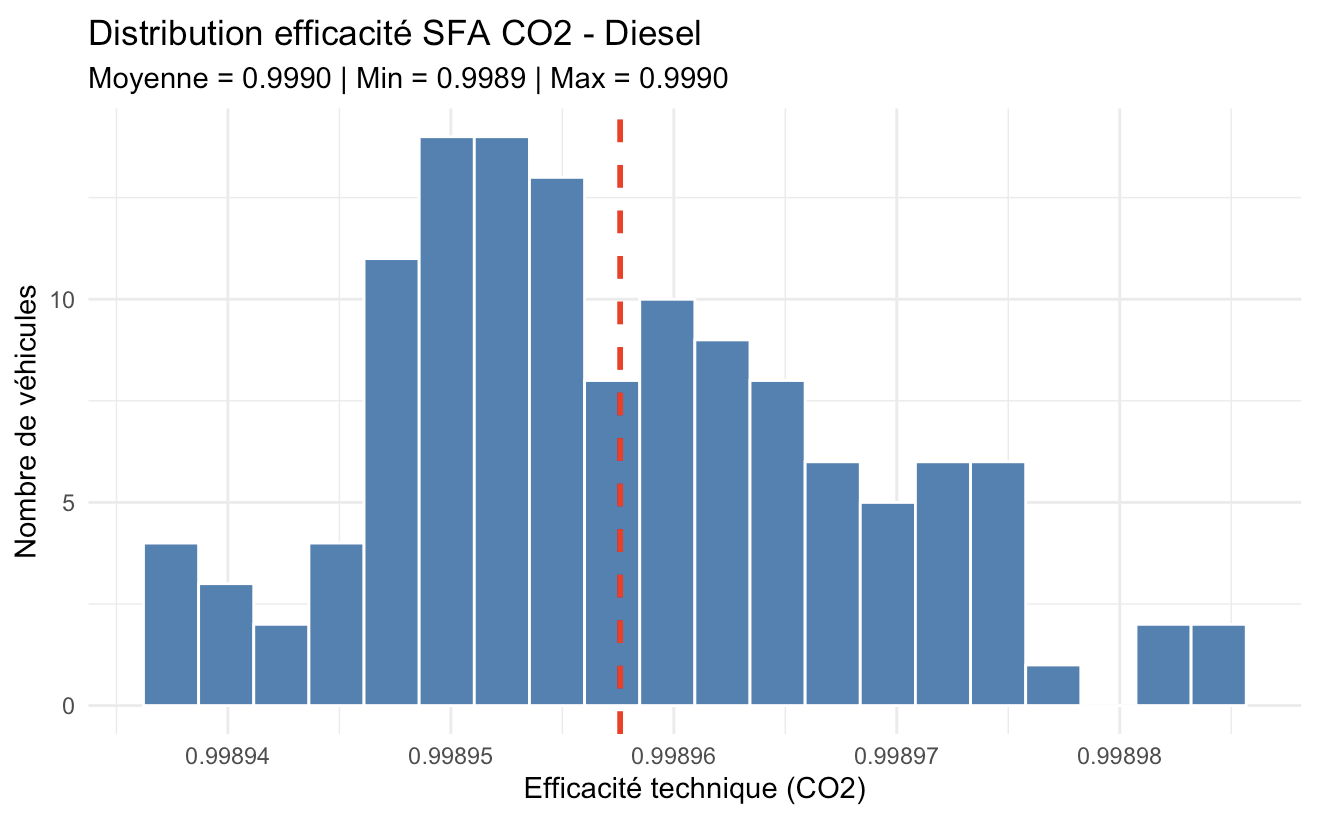
\includegraphics[width=0.74\textwidth]{résultats/SFA_CO2_Diesel.png}
    \caption{Distribution SFA de l'efficacité CO2 -- motorisation Diesel.}
    \label{fig:sfa_co2_diesel}
\end{figure}

Dans le prolongement de l'analyse des motorisations à essence, le modèle SFA appliqué aux véhicules Diesel révèle une dynamique strictement similaire concernant les émissions de CO2. L'histogramme de la distribution de l'efficacité technique affiche une moyenne de 0.9990, avec des valeurs extrêmes confinées entre 0.9989 et 0.9990. À nouveau, bien que la représentation graphique étire artificiellement l'axe des abscisses pour faire apparaître une distribution en cloche, la projection de ces résultats sur notre échelle de référence absolue (de 0 à 1) met en évidence une absence quasi totale de variance.

\vspace{0.6em}

Interprétation technologique : Ce constat confirme que la motorisation Diesel, tout comme l'Essence, a atteint son asymptote de développement en matière de rendement énergétique pur. L'ensemble des véhicules Diesel de notre échantillon se situe sur la frontière d'efficience maximale (score extrêmement proche de 1). Il n'existe donc pas, sur le marché européen actuel, de constructeurs proposant des moteurs Diesel thermiques purs qui soient significativement sous-optimisés par rapport à l'état de l'art technologique.

\vspace{0.6em}

Sur le plan analytique, ce résultat renforce la thèse centrale de notre étude développée dans la première partie : puisque l'inefficacité technique intrinsèque du groupe motopropulseur est virtuellement nulle, les variations des émissions absolues de CO2 mesurées lors de l'homologation sont exclusivement imputables aux contraintes physiques. Le volume de CO2 rejeté par un véhicule Diesel moderne est le reflet direct et incompressible de sa masse (et donc de l'énergie cinétique requise pour vaincre l'inertie) ainsi que de sa résistance aérodynamique et au roulement. Cette observation empirique confirme la futilité d'espérer des gains environnementaux substantiels (sur le seul prisme du CO2) par la micro-ingénierie des moteurs thermiques, sans une politique de réduction drastique de la masse des véhicules.

\subsubsection{Efficacité technique CO2 des motorisations Hybrides Rechargeables : L'hétérogénéité des choix architecturaux}

\begin{figure}[H]
    \centering
    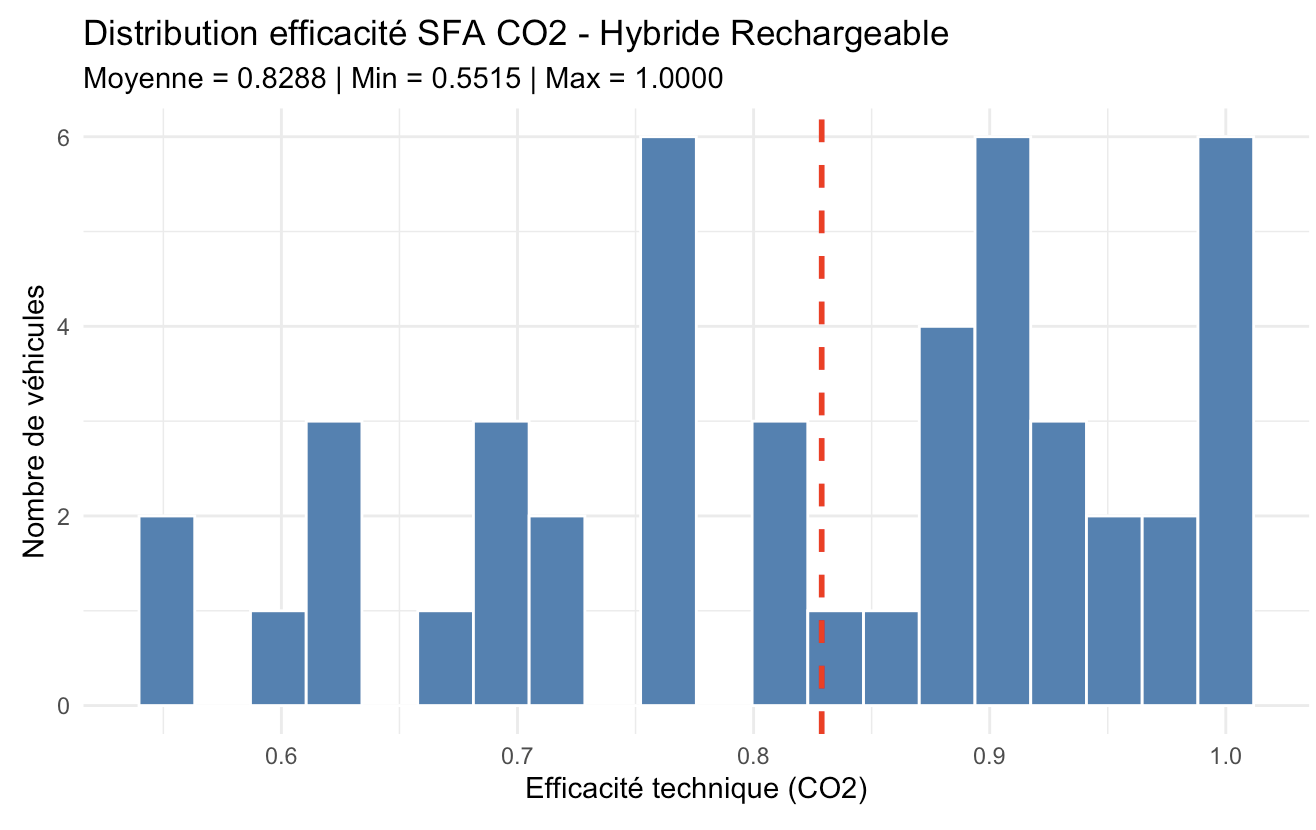
\includegraphics[width=0.74\textwidth]{résultats/SFA_CO2_Hybrides_Rechargeables.png}
    \caption{Distribution SFA de l'efficacité CO2 -- Hybrides Rechargeables.}
    \label{fig:sfa_co2_phev}
\end{figure}

Le contraste avec les motorisations thermiques pures est saisissant. L'application du modèle SFA aux véhicules Hybrides Rechargeables (PHEV) révèle une dynamique d'efficience radicalement différente. L'histogramme de la distribution s'étale très largement sur notre échelle de référence (de 0 à 1), avec une moyenne chutant à 0.8288 et des valeurs s'éparpillant d'un minimum alarmant de 0.5515 jusqu'à la frontière optimale de 1.0000.

\vspace{0.6em}

Interprétation technologique : Cette très forte variance traduit une absence de standardisation technologique et une immense hétérogénéité dans les choix d'ingénierie des constructeurs. Contrairement aux moteurs essence ou diesel dont le développement a atteint un plafond de verre thermodynamique, l'hybridation rechargeable permet une multitude d'architectures combinatoires (taille de la batterie, puissance du moteur électrique par rapport au moteur thermique, stratégies de gestion des flux d'énergie).

\vspace{0.6em}

L'étalement des scores d'efficacité met en exergue deux réalités industrielles distinctes :

\vspace{0.6em}

\begin{itemize}
    \item Les véhicules efficients (scores proches de 1) : Ils témoignent d'une intégration technologique optimale. Ces modèles exploitent au mieux la synergie entre les deux motorisations pour minimiser le CO2, au-delà de ce que leur simple masse ou aérodynamisme laisserait présager.

    \vspace{0.5em}

    \item Les véhicules structurellement inefficients (scores inférieurs à 0.75) : La présence d'une "queue de distribution" aussi marquée sur la gauche du graphique est révélatrice des stratégies d'optimisation artificielle en laboratoire détaillées dans la première partie de notre étude. Notre modèle SFA contrôlant ex-ante l'effet pénalisant du poids et de la carrosserie, le faible score de ces véhicules indique que leur groupe motopropulseur hybride est intrinsèquement sous-performant. Il s'agit typiquement de véhicules conçus comme des "véhicules de conformité" (souvent de lourds SUV dotés de batteries sous-dimensionnées) dont l'architecture complexe sert davantage à exploiter les failles du cycle d'homologation WLTP qu'à offrir une réelle efficience énergétique en conditions réelles.
\end{itemize}

\vspace{0.6em}

Ce résultat empirique valide notre hypothèse initiale : l'ajout d'un système hybride rechargeable ne garantit en rien une efficience environnementale absolue. L'étiquette "PHEV" masque des disparités d'ingénierie massives, où cohabitent des véhicules à la pointe de l'optimisation et des modèles dont la complexité technologique peine à masquer une profonde inefficacité structurelle.

\subsubsection{Efficacité technique CO2 des motorisations Hybrides Non-Rechargeables : La fracture technologique masquée par la nomenclature}

\begin{figure}[H]
    \centering
    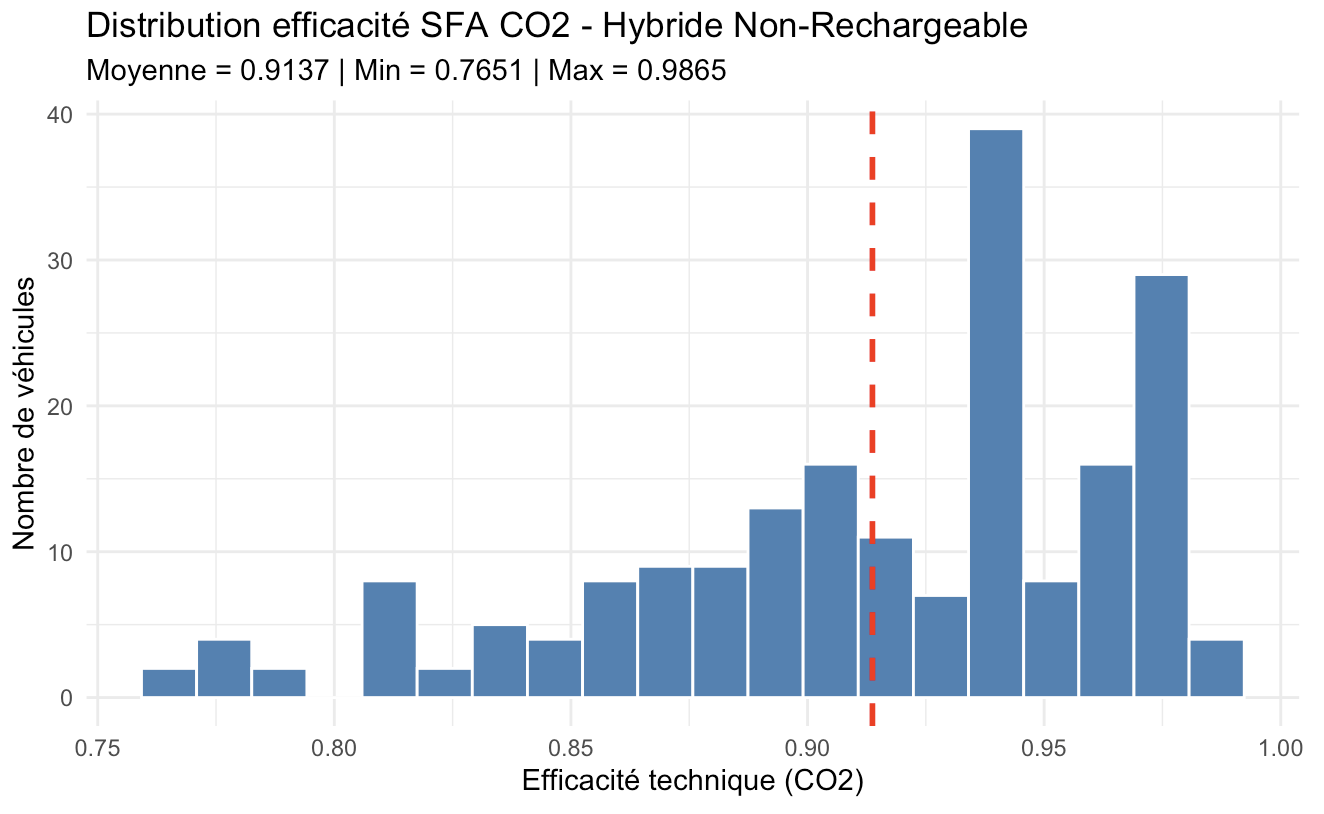
\includegraphics[width=0.74\textwidth]{résultats/SFA_CO2_Hybrides_non_Rechargeables.png}
    \caption{Distribution SFA de l'efficacité CO2 -- Hybrides Non-Rechargeables.}
    \label{fig:sfa_co2_hev}
\end{figure}

L'analyse de la distribution de l'efficacité technique pour les véhicules Hybrides Non-Rechargeables révèle une structure particulièrement instructive. L'histogramme affiche une moyenne de 0.9137, avec des valeurs s'étalant de 0.7651 à un maximum de 0.9865 sur notre échelle absolue de 0 à 1.

\vspace{0.6em}

Contrairement aux motorisations thermiques pures (où la variance était nulle) ou aux hybrides rechargeables (où la distribution était chaotique), nous observons ici une distribution clairement multimodale, caractérisée par plusieurs pics distincts : une forte concentration de véhicules très efficients (scores compris entre 0.93 et 0.98) et une "traîne" asymétrique de véhicules nettement moins performants (scores s'étalant de 0.76 à 0.90).

\vspace{0.6em}

Interprétation technologique et réglementaire : Cette distribution fracturée est la traduction empirique d'un biais de nomenclature majeur dans l'homologation automobile : le regroupement sous la même étiquette administrative "Hybride Non-Rechargeable" de deux architectures technologiques fondamentalement différentes. Le modèle SFA, en contrôlant l'effet de la masse et de la puissance, parvient à isoler et à séparer mathématiquement ces deux mondes :

\vspace{0.6em}

\begin{itemize}
    \item L'hybridation complète ("Full Hybrid" ou HEV) : Le pic de haute efficacité (se rapprochant de la frontière de 1) correspond aux véritables systèmes hybrides. Ces véhicules disposent d'un moteur électrique opérant sous haute tension, capable de mouvoir le véhicule de manière autonome à basse vitesse et de soulager significativement le moteur thermique lors des phases de forte charge (accélération). Leur architecture permet d'atteindre une efficience de conversion énergétique remarquable compte tenu de leur masse.

    \vspace{0.5em}

    \item La micro-hybridation ("Mild Hybrid" ou MHEV) : La partie gauche de la distribution (scores inférieurs à 0.90) regroupe les véhicules dotés d'une hybridation légère (généralement un réseau 48V couplé à un alterno-démarreur). Ces systèmes sont incapables de propulser seuls le véhicule. L'assistance électrique y est marginale.
\end{itemize}

\vspace{0.6em}

Ce résultat fait directement écho aux stratégies de conformité réglementaire abordées dans la première partie de notre rapport. Face à la pression de la norme CAFE, de nombreux constructeurs ont opté pour la micro-hybridation, une solution technologique peu coûteuse permettant d'abaisser artificiellement de quelques grammes les émissions de CO2 sur le cycle WLTP pour éviter les pénalités financières. Cependant, notre analyse SFA démontre que, ramenés à leur masse et à leur puissance, ces véhicules "Mild Hybrid" restent structurellement inefficients. Ils s'éloignent de la frontière technologique optimale, prouvant que l'étiquette "Hybride" ne garantit pas une efficacité systémique homogène au sein de cette catégorie.

\subsection{Efficacité technique relative aux Hydrocarbures (HC) : L'homogénéité du post-traitement}

Après avoir analysé l'efficacité technique liée aux rejets de CO2, notre étude par frontière stochastique se penche sur le traitement des hydrocarbures imbrûlés (HC).

\vspace{0.6em}

Il convient tout d'abord de justifier l'absence de modélisation SFA des HC pour les motorisations Diesel dans cette section. Comme abordé dans notre revue de la chimie du moteur, un moteur Diesel fonctionne de manière intrinsèque en excès d'air (mélange pauvre). Cette abondance d'oxygène dans la chambre de combustion garantit une oxydation quasi totale des hydrocarbures à la source. Par conséquent, les rejets de HC par les véhicules Diesel modernes sont si infimes qu'ils ne constituent plus un défi d'ingénierie distinct. Dans les bases de données d'homologation, ils sont d'ailleurs fréquemment agrégés aux oxydes d'azote sous la norme combinée (HC+NOx) ou tout simplement exclus des mesures spécifiques exploitables pour une modélisation SFA robuste.

\subsubsection{Efficacité technique HC des motorisations Essence : L'universalité du traitement catalytique}

\begin{figure}[H]
    \centering
    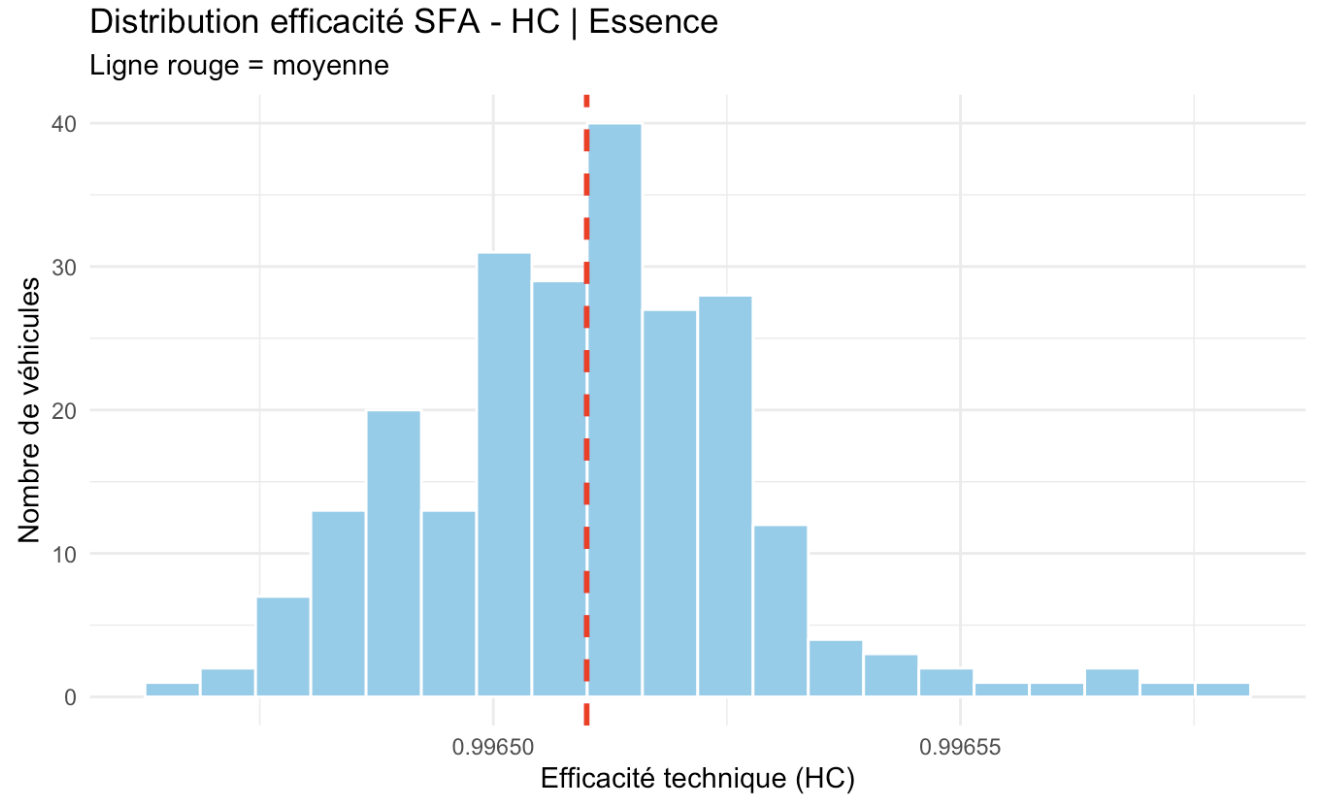
\includegraphics[width=0.74\textwidth]{résultats/SFA_HC_Essence.png}
    \caption{Distribution SFA de l'efficacité HC -- motorisation Essence.}
    \label{fig:sfa_hc_essence}
\end{figure}

L'analyse de la distribution de l'efficacité technique pour le traitement des HC sur le sous-échantillon des véhicules à Essence révèle un phénomène statistique désormais familier. Si l'histogramme présente une forme classique en cloche, la lecture de l'axe des abscisses est à nouveau révélatrice : la distribution est centrée sur une moyenne d'environ 0.9951, avec des bornes d'une étroitesse extrême (de 0.99650 à 0.99655). Ramenée à notre échelle absolue de référence allant de 0 à 1, la variance de cet échantillon est microscopique. L'intégralité des véhicules à essence testés se situe sur la frontière d'efficience maximale, ou à une fraction infinitésimale de celle-ci.

\vspace{0.6em}

Interprétation technologique : Ce résultat empirique démontre que le traitement des hydrocarbures imbrûlés n'est plus un élément de différenciation technologique entre les constructeurs pour les moteurs à allumage commandé. Il valide l'efficacité universelle et absolue des systèmes de post-traitement modernes, en l'occurrence les catalyseurs à trois voies.

\vspace{0.6em}

Grâce à l'utilisation de métaux nobles tels que le Platine et le Palladium, la réaction d'oxydation transformant les HC en vapeur d'eau et en CO2 est aujourd'hui maîtrisée à la perfection par l'ensemble de l'industrie. Les infimes variations observées (de l'ordre de la troisième ou quatrième décimale) ne traduisent pas une différence d'architecture moteur, mais reflètent très probablement des écarts marginaux dans la vitesse de montée en température du pot catalytique (le light-off) lors des premières secondes du cycle d'homologation à froid. En régime établi, l'inefficacité technique sur ce polluant est nulle.

\subsubsection{Efficacité technique HC des motorisations Hybrides : La neutralisation des architectures par la post-combustion}

\begin{figure}[H]
    \centering
    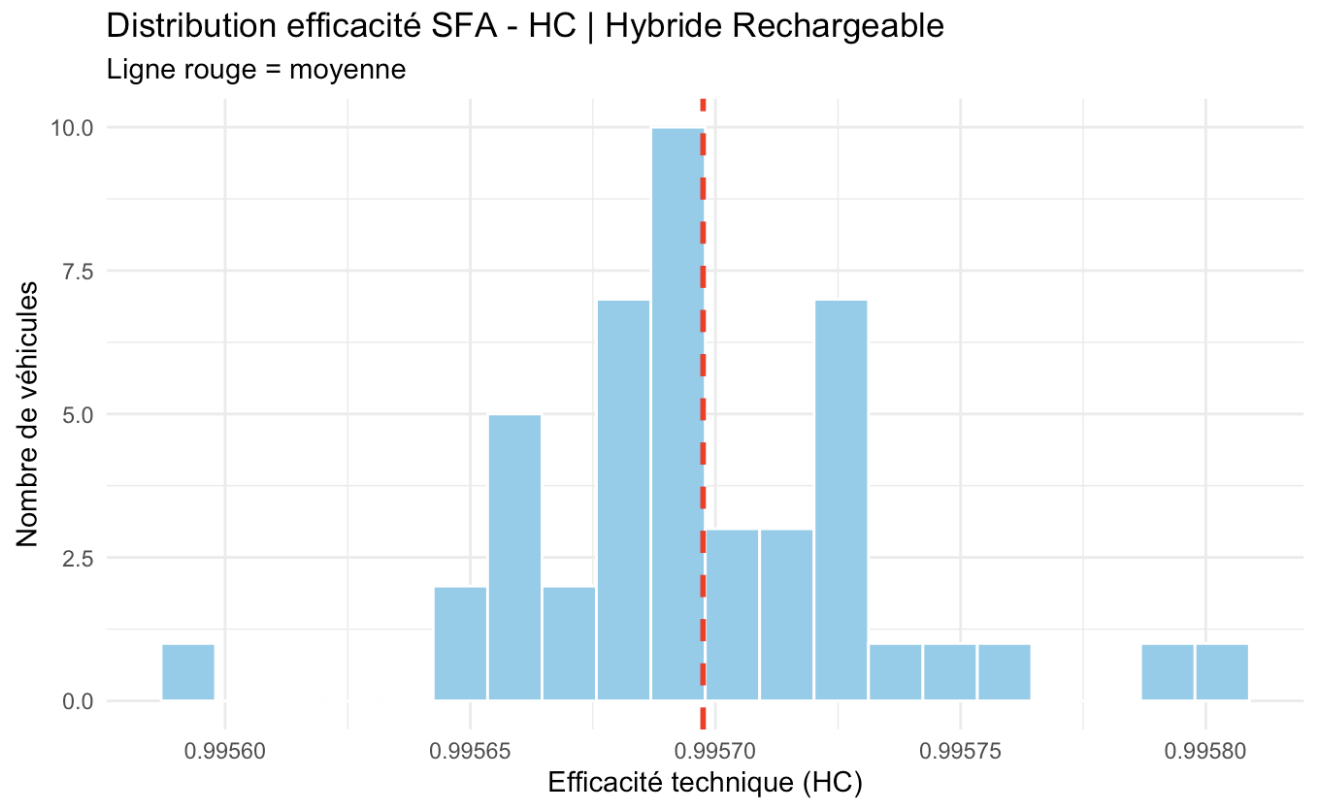
\includegraphics[width=0.74\textwidth]{résultats/SFA_HC_Hybrides_Rechargeables.png}
    \caption{Distribution SFA de l'efficacité HC -- Hybrides Rechargeables.}
    \label{fig:sfa_hc_phev}
\end{figure}

\begin{figure}[H]
    \centering
    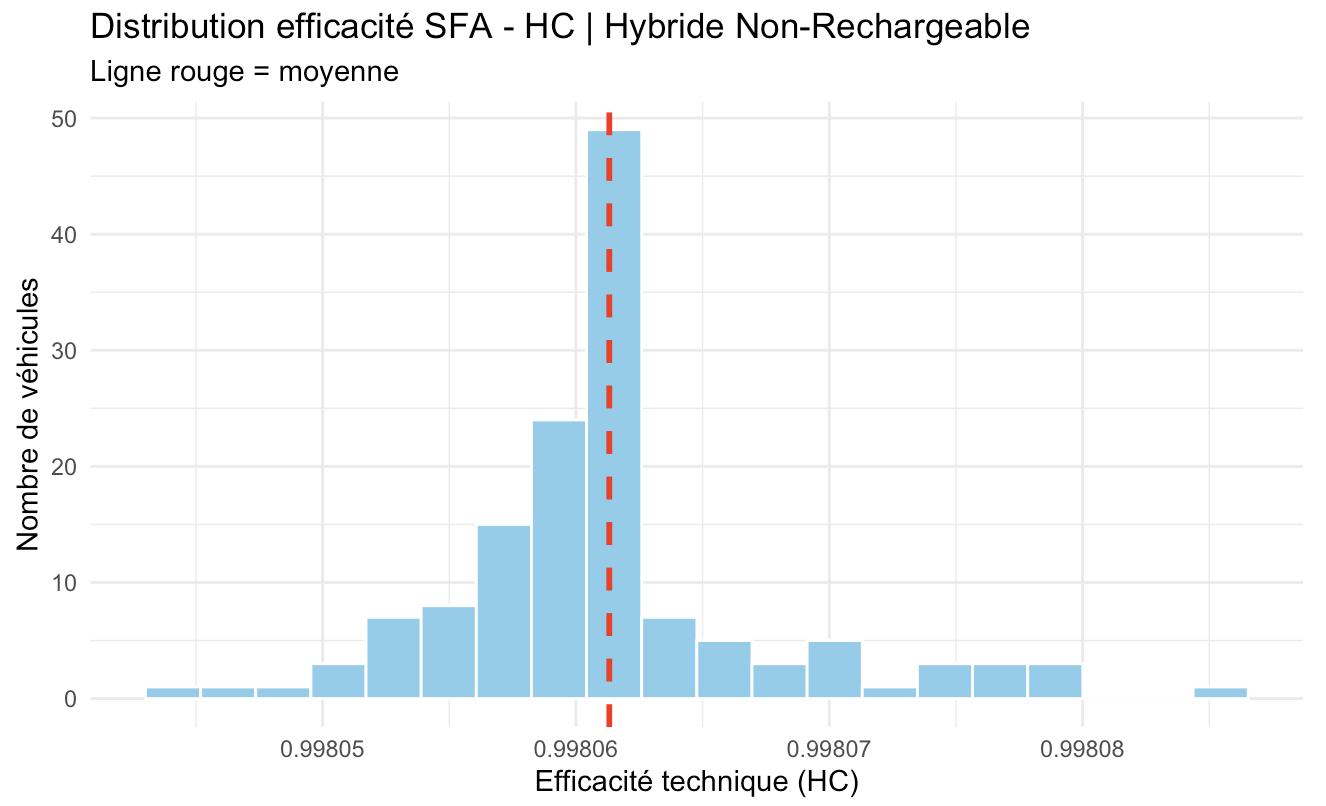
\includegraphics[width=0.74\textwidth]{résultats/SFA_HC_Hybrides_non_Rechargeables.png}
    \caption{Distribution SFA de l'efficacité HC -- Hybrides Non-Rechargeables.}
    \label{fig:sfa_hc_hev}
\end{figure}

Afin d'alléger l'analyse et de souligner la convergence des résultats, nous traitons conjointement l'efficacité technique relative aux hydrocarbures (HC) pour les motorisations Hybrides Rechargeables (PHEV) et Non-Rechargeables (HEV).

\vspace{0.6em}

L'observation des deux histogrammes révèle une dynamique strictement identique à celle constatée sur les motorisations thermiques à essence, et ce, malgré les profondes différences d'architecture électrique de ces véhicules.

\vspace{0.6em}

\begin{itemize}
    \item Pour les Hybrides Rechargeables, la moyenne s'établit à 0.9957, avec des valeurs confinées dans un intervalle microscopique (de 0.9956 à 0.9958).

    \vspace{0.5em}

    \item Pour les Hybrides Non-Rechargeables, le constat est le même : une moyenne de 0.9980 et une distribution écrasée entre 0.9980 et 0.9981. Rappelons que notre échelle d'efficacité absolue s'étend de 0 à 1. Les courbes en cloche affichées par les graphiques ne sont que des artefacts visuels liés au zoom automatique des axes. Dans la réalité mathématique de notre modèle, la variance est virtuellement nulle : l'intégralité du parc automobile hybride se situe sur la frontière technologique optimale concernant le traitement des HC.
\end{itemize}

\vspace{0.6em}

Interprétation technologique : Ce résultat empirique est fondamental pour notre étude car il démontre que la chimie supplante l'architecture mécanique.

\vspace{0.6em}

Lors de notre analyse du CO2, nous avions mis en évidence une très forte hétérogénéité (des distributions étalées ou multimodales) liée aux choix d'hybridation (micro-hybridation vs hybridation complète, taille de la batterie). Ici, pour le polluant HC, ces disparités architecturales s'effacent totalement. Qu'un véhicule dispose d'un modeste réseau 48V ou d'une imposante batterie rechargeable, son moteur thermique à allumage commandé reste équipé d'un pot catalytique à trois voies dont la capacité d'oxydation est universellement performante. En conclusion, la maîtrise industrielle des réactions d'oxydation par catalyse est telle qu'elle garantit une efficience maximale et homogène pour l'élimination des hydrocarbures imbrûlés, rendant ce polluant imperméable aux variations de conception des systèmes hybrides.

\subsection{Efficacité technique relative aux Oxydes d'Azote (NOx) : Le véritable juge de paix technologique}

La modélisation de l'efficacité technique franchit un cap décisif avec l'analyse des oxydes d'azote (NOx). Si notre étude a démontré que le CO2 était une fatalité physique et les HC un problème chimique largement résolu au démarrage, le traitement des NOx révèle les véritables arbitrages d'ingénierie et financiers opérés par les constructeurs.

\subsubsection{Efficacité technique NOx des motorisations Essence : Le grand écart technologique et financier}

\begin{figure}[H]
    \centering
    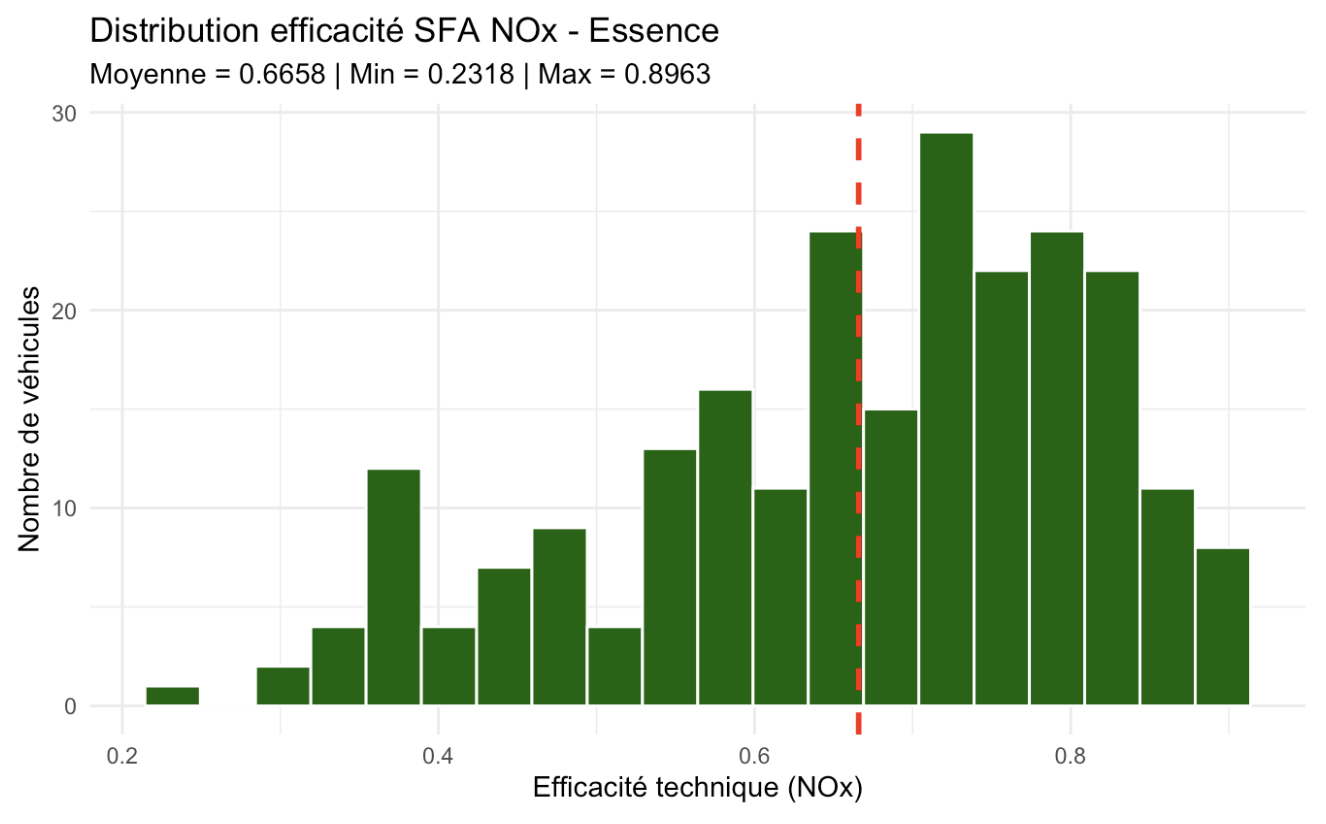
\includegraphics[width=0.74\textwidth]{résultats/SFA_Nox_Essence.png}
    \caption{Distribution SFA de l'efficacité NOx -- motorisation Essence.}
    \label{fig:sfa_nox_essence}
\end{figure}

Le graphique de distribution SFA pour les véhicules à motorisation Essence marque une rupture totale avec les constats précédents. Contrairement au resserrement microscopique observé pour le CO2 et les HC, l'histogramme des NOx révèle une immense hétérogénéité.

\vspace{0.6em}

Sur notre échelle absolue allant de 0 à 1, la variance est ici spectaculaire : l'efficacité technique s'étale d'un minimum critique de 0.2318 à un maximum de 0.8963, avec une moyenne s'établissant à 0.6658. L'échantillon est largement dispersé, mettant en évidence la coexistence de véhicules très performants et de modèles structurellement inefficients pour contenir ce polluant à masse et puissance égales.

\vspace{0.6em}

Interprétation technologique et économique : Cette très forte variance traduit le fait que l'élimination des NOx n'est pas une commodité standardisée, mais un défi complexe qui cristallise les compromis industriels.

\vspace{0.6em}

Ce constat s'explique par deux facteurs fondamentaux détaillés dans notre revue théorique :

\vspace{0.6em}

\begin{itemize}
    \item L'arbitrage financier sur les métaux critiques : Bien que tous les véhicules à essence soient équipés d'un pot catalytique "3 voies", la réduction des oxydes d'azote en diazote inoffensif (N2) repose spécifiquement sur l'utilisation du Rhodium. Or, ce métal précieux est l'un des plus chers au monde, soumis à une volatilité extrême de ses cours. Le coût des métaux précieux dans un catalyseur impactant directement le prix de revient du véhicule, l'efficacité du système dépend largement du budget alloué par le constructeur. Les véhicules affichant un score SFA médiocre (autour de 0.3 ou 0.4) sont symptomatiques de systèmes de post-traitement sous-dimensionnés en métaux réducteurs, incapables d'absorber les pics d'émissions lors des fortes charges motrices.

    \vspace{0.5em}

    \item Le compromis fatal avec le CO2 (La fenêtre Lambda) : La réaction chimique de réduction des NOx est extrêmement fragile. Elle exige que le moteur fonctionne avec un mélange parfait. Dès que l'ingénierie opte pour un mélange légèrement "pauvre" (excès d'air) pour réduire la consommation de carburant et obtenir de bons scores en CO2 lors de l'homologation, le catalyseur perd quasi instantanément sa capacité à traiter les NOx. L'étalement des scores d'efficacité reflète donc les choix de cartographie moteur : sacrifier la destruction des NOx pour optimiser le rendement thermique et éviter les sanctions réglementaires liées au CO2.
\end{itemize}

\vspace{0.6em}

En somme, ce modèle SFA démontre que sur le segment de l'essence, la dépollution des NOx est une variable d'ajustement. Elle sépare les véhicules bénéficiant d'une ingénierie de pointe sans compromis, de ceux contraints par des impératifs économiques ou par l'obsession réglementaire de la baisse du dioxyde de carbone.

\subsubsection{Efficacité technique NOx des motorisations Diesel : La fracture des systèmes de post-traitement}

\begin{figure}[H]
    \centering
    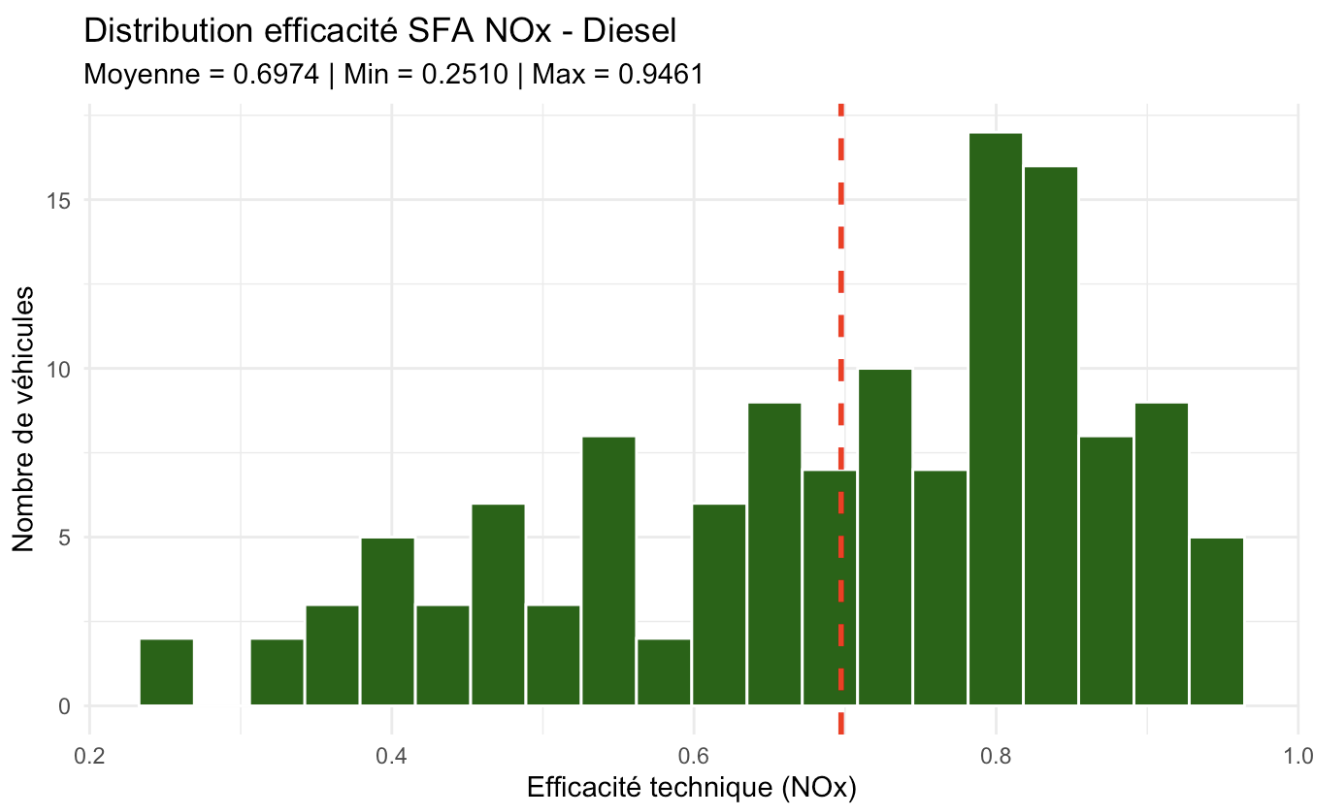
\includegraphics[width=0.74\textwidth]{résultats/SFA_Nox_Diesel.png}
    \caption{Distribution SFA de l'efficacité NOx -- motorisation Diesel.}
    \label{fig:sfa_nox_diesel}
\end{figure}

Dans la continuité de l'analyse des motorisations à essence, la distribution SFA relative aux véhicules Diesel confirme la difficulté systémique du traitement des oxydes d'azote, tout en mettant en lumière des dynamiques industrielles qui lui sont propres.

\vspace{0.6em}

L'histogramme présente une très forte hétérogénéité des performances. Sur notre échelle absolue (de 0 à 1), la moyenne s'établit à 0.6974, avec des scores extrêmement dispersés, allant d'un minimum critique de 0.2510 à un maximum de 0.9461. Cette large variance démontre que l'efficience sur ce polluant est loin d'être un acquis technologique standardisé au sein du parc automobile Diesel.

\vspace{0.6em}

Interprétation technologique : Le transfert vers la post-combustion. La variance observée ici s'explique par les contraintes thermodynamiques inhérentes au cycle Diesel. Ce type de moteur fonctionne structurellement en excès d'air et nécessite, pour mouvoir des véhicules de plus en plus lourds, des pressions de combustion très élevées. Ces conditions entraînent mécaniquement une élévation de la température interne au-delà de 1400 degC, favorisant massivement la formation de NOx "à la source" via la réaction de Zeldovich.

\vspace{0.6em}

Par conséquent, l'écart d'efficacité technique mesuré par notre modèle SFA ne reflète pas une optimisation de la combustion dans le cylindre, mais évalue presque exclusivement la capacité et le coût des dispositifs de post-traitement installés à l'échappement. La large dispersion des scores illustre une véritable fracture technologique dictée par les choix d'investissement des constructeurs :

\vspace{0.6em}

\begin{itemize}
    \item Les véhicules de haute efficience (scores > 0.80) : Ce groupe, très visible sur la droite du graphique, correspond aux modèles équipés de systèmes SCR (Selective Catalytic Reduction) de pointe. L'injection d'urée (AdBlue) permet de neutraliser efficacement les NOx, même sous forte charge. Cependant, cette technologie représente un coût d'ingénierie majeur et nécessite l'embarquement de réservoirs supplémentaires qui alourdissent le véhicule, illustrant parfaitement le cercle vicieux entre masse, recherche de puissance et systèmes de dépollution mis en évidence dans notre revue de littérature.
\end{itemize}

\vspace{0.6em}

\begin{itemize}
    \item Les véhicules structurellement inefficients (scores < 0.60) : La longue traîne gauche de la distribution regroupe les véhicules s'appuyant sur des technologies de dépollution moins onéreuses (telles que les pièges à NOx / LNT ou une forte dépendance à la seule vanne EGR). Ces systèmes plus économiques saturent rapidement lors des variations de charge dynamiques, entraînant une chute drastique de l'efficacité globale face aux exigences physiques imposées par la masse du véhicule.
\end{itemize}

\vspace{0.6em}

Ce résultat démontre empiriquement que, pour le Diesel, la maîtrise des émissions de NOx n'est pas limitée par un plafond technologique absolu, mais par un plafond économique. L'efficacité environnementale est ici directement corrélée à la complexité et au coût du système de post-traitement embarqué

\subsubsection{Efficacité technique NOx des motorisations Hybrides Rechargeables : Le biais du cycle d'homologation}

\begin{figure}[H]
    \centering
    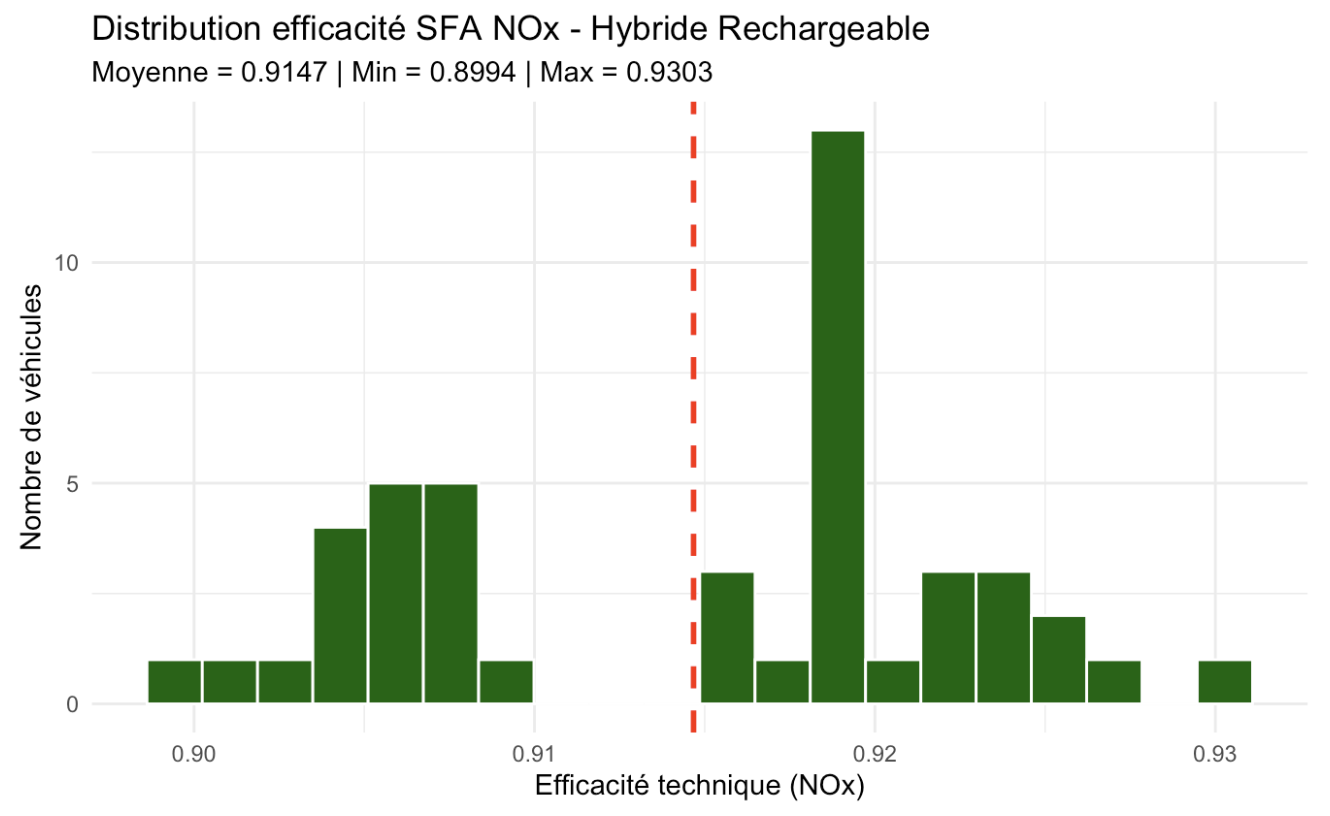
\includegraphics[width=0.74\textwidth]{résultats/SFA_Nox_Hybrides_Rechargeables.png}
    \caption{Distribution SFA de l'efficacité NOx -- Hybrides Rechargeables.}
    \label{fig:sfa_nox_phev}
\end{figure}

L'analyse de la distribution SFA des oxydes d'azote pour les Hybrides Rechargeables (PHEV) tranche radicalement avec l'hétérogénéité observée sur les motorisations thermiques classiques. L'histogramme révèle une variance extrêmement faible : l'efficacité technique est concentrée dans un intervalle très restreint, s'étendant d'un minimum de 0.8994 à un maximum de 0.9303 (pour une moyenne de 0.9147).

\vspace{0.6em}

Interprétation technologique et réglementaire : Sur notre échelle absolue allant de 0 à 1, l'ensemble de ce sous-échantillon apparaît comme hautement et uniformément efficient. Toutefois, cette homogénéité de façade s'explique davantage par les modalités du protocole d'homologation WLTP que par une rupture technologique dans les systèmes de dépollution. En effet, lors des tests officiels, ces véhicules parcourent une part significative du cycle en mode 100 \% électrique. De plus, lorsque le moteur thermique est sollicité, l'assistance de la batterie permet de lisser les phases de fortes charges transitoires (les accélérations brusques), qui sont précisément les conditions critiques favorisant l'explosion des rejets de NOx à la source. Le modèle SFA observe donc des émissions à l'échappement artificiellement basses au regard de la masse imposante de ces véhicules hybrides, et leur attribue mécaniquement d'excellents scores.

\vspace{0.6em}

Ce résultat illustre parfaitement les limites de la norme actuelle, qui tend à masquer les véritables capacités (ou faiblesses) de traitement des gaz d'échappement de ces véhicules en situation de batterie déchargée.

\subsubsection{Efficacité technique NOx des motorisations Hybrides Non-Rechargeables : La polarisation extrême des architectures}

\begin{figure}[H]
    \centering
    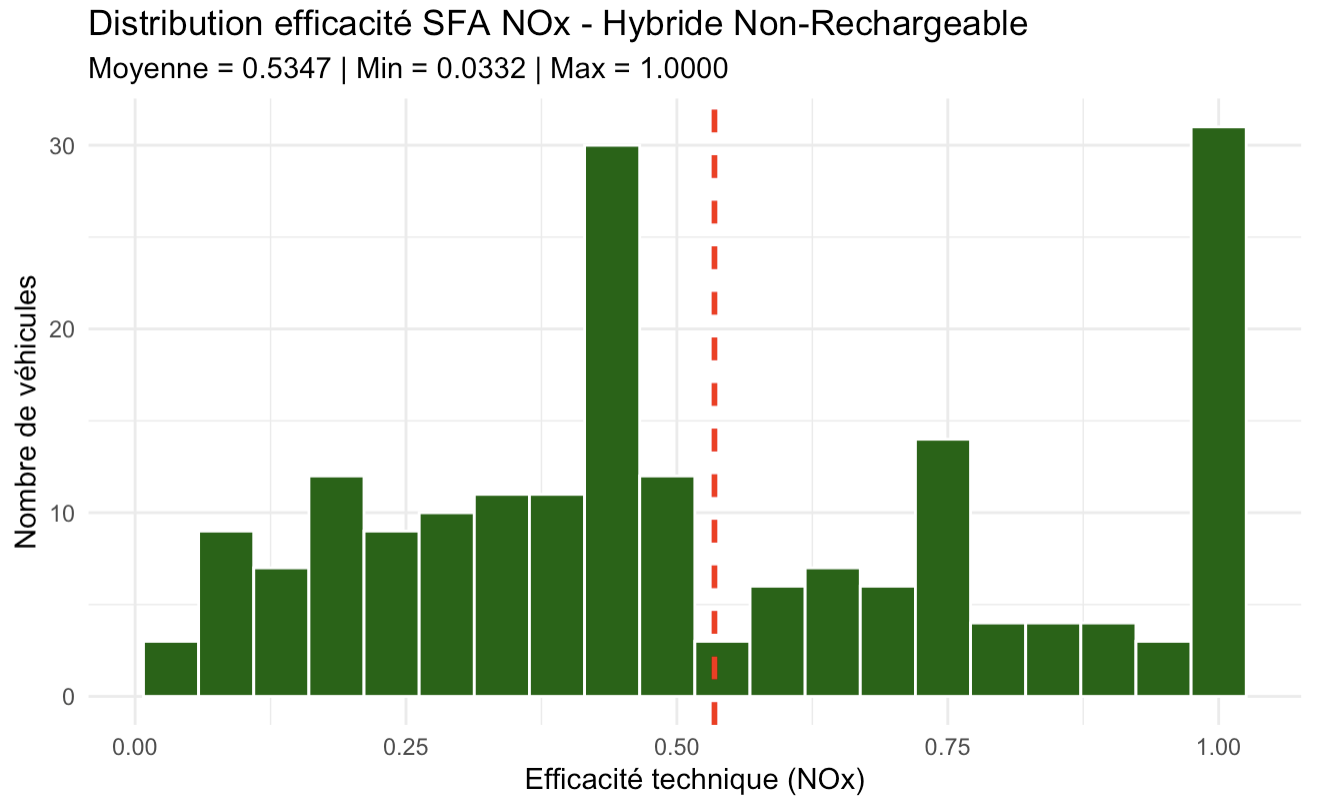
\includegraphics[width=0.74\textwidth]{résultats/SFA_Nox_Hybrides_non_Rechargeables.png}
    \caption{Distribution SFA de l'efficacité NOx -- Hybrides Non-Rechargeables.}
    \label{fig:sfa_nox_hev}
\end{figure}

Le graphique de distribution SFA des oxydes d'azote pour les véhicules Hybrides Non-Rechargeables constitue le résultat le plus clivé de notre étude empirique. Avec une moyenne chutant à 0.5347 et des scores s'étalant d'un minimum critique de 0.0332 à la perfection technologique de 1.0000, l'histogramme dévoile une fracture spectaculaire au sein de cette même catégorie administrative.

\vspace{0.6em}

Interprétation technologique : Le révélateur des limites de la micro-hybridation. Cette distribution, fortement polarisée entre un pic absolu d'efficience (à 1.00) et un vaste regroupement de véhicules très inefficients (en deçà de 0.50), corrobore l'hétérogénéité architecturale déjà identifiée lors de l'analyse du CO2, mais l'amplifie de manière critique sur le plan sanitaire :

\vspace{0.6em}

\begin{itemize}

    \item Le pic de perfection (score de 1.00) : Il isole les systèmes d'hybridation complète ("Full Hybrid"). Grâce à un moteur électrique suffisamment puissant pour absorber les pics d'efforts lors des accélérations, le moteur thermique est préservé des phases de forte charge. Cette synergie empêche mécaniquement l'élévation des températures internes au-delà de 1400 degC, bloquant ainsi la formation des NOx à la source via la réaction de Zeldovich.
\end{itemize}

\vspace{0.6em}

\begin{itemize}
    \item La forte inefficacité (scores < 0.60) : Ce large groupe démasque les systèmes de micro-hybridation ("Mild Hybrid"). L'assistance électrique y étant trop faible pour soulager significativement le moteur thermique en charge, ce dernier chauffe et génère des pics de NOx que le système d'échappement standard peine à filtrer de manière optimale.
\end{itemize}

\vspace{0.6em}

En conclusion, si la micro-hybridation constitue un outil à bas coût pour les constructeurs afin d'optimiser artificiellement les rejets de CO2 lors des cycles d'homologation, notre modèle SFA révèle qu'elle échoue lourdement sur le front sanitaire des oxydes d'azote, soulignant les limites environnementales de ces architectures de compromis.

\subsection{Efficacité technique combinée (HC+NOx) : La confirmation de l'hégémonie des oxydes d'azote}

\begin{figure}[H]
    \centering
    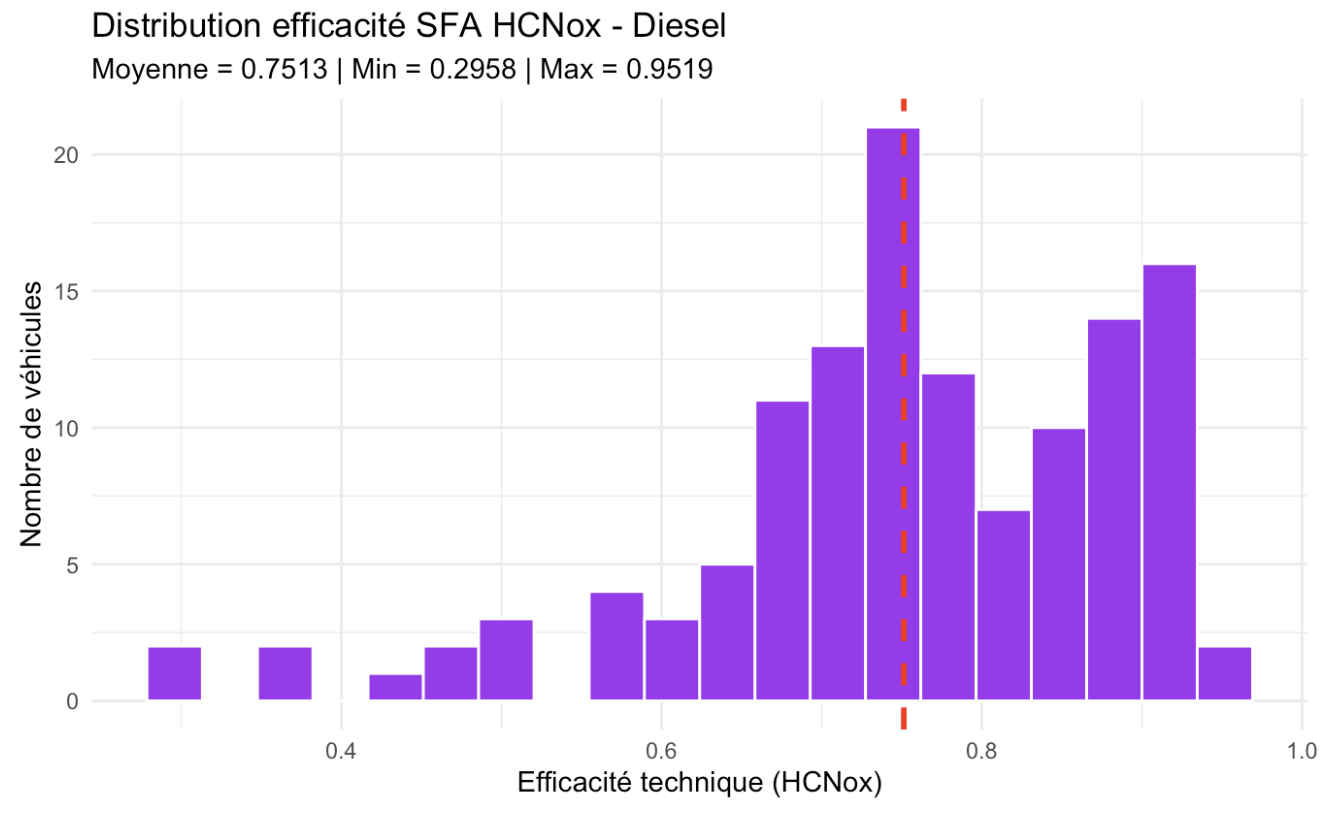
\includegraphics[width=0.74\textwidth]{résultats/SFA_HCNox_Diesel.png}
    \caption{Distribution SFA de l'efficacité combinée (HC + NOx) -- Diesel.}
    \label{fig:sfa_hcnox_diesel}
\end{figure}

\begin{figure}[H]
    \centering
    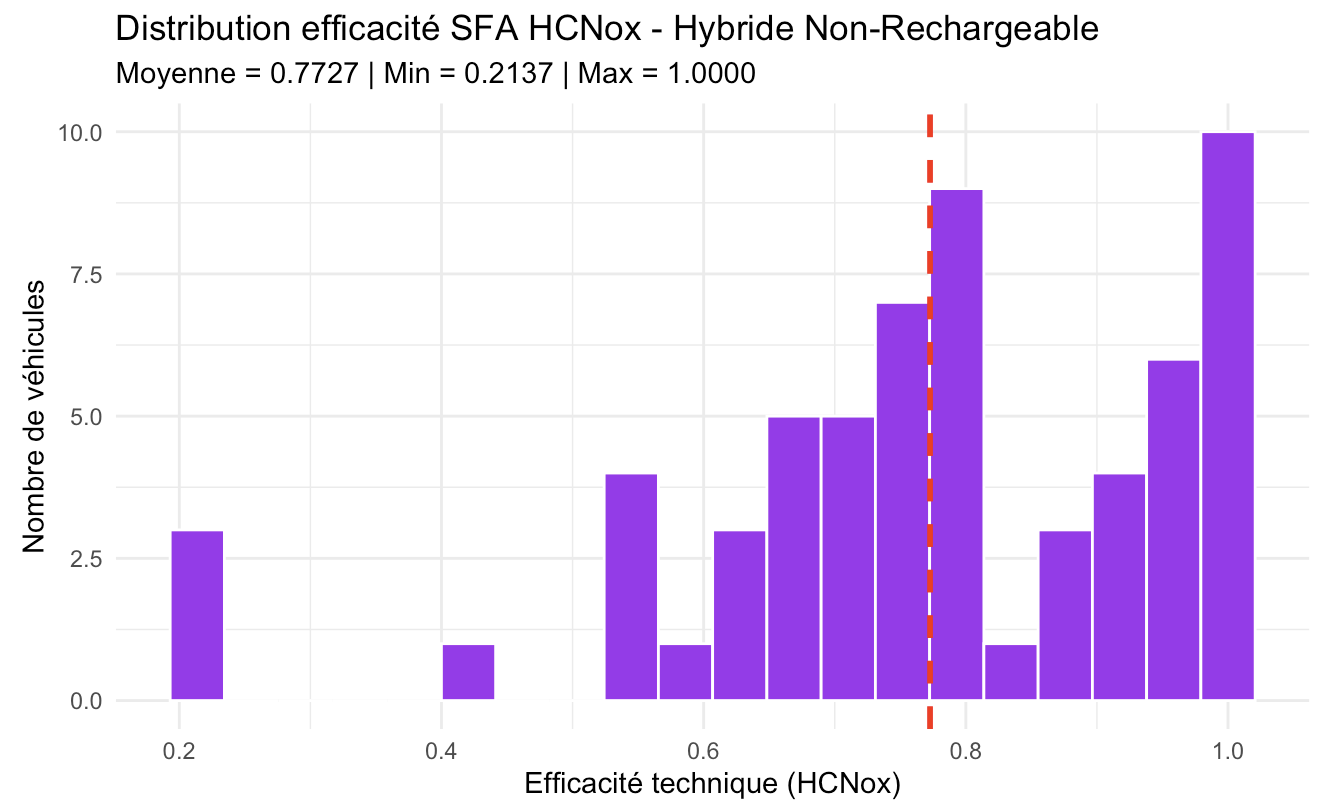
\includegraphics[width=0.74\textwidth]{résultats/SFA_HCNox_Hybrides_non_Rechargeables.png}
    \caption{Distribution SFA de l'efficacité combinée (HC + NOx) -- Hybrides Non-Rechargeables.}
    \label{fig:sfa_hcnox_hev}
\end{figure}

L'analyse de la norme combinée HC+NOx, fréquemment utilisée dans l'homologation européenne pour évaluer globalement les polluants locaux, offre une synthèse particulièrement éclairante de nos résultats SFA.

\vspace{0.6em}

Comme démontré à la section 8.5, le traitement des hydrocarbures (HC) atteint une efficacité quasi parfaite et universelle grâce à la post-combustion pour les motorisations hybrides, et s'avère naturellement marginal pour les motorisations Diesel opérant en excès d'air. Par conséquent, la variance que l'on observe sur cet indicateur combiné masque une asymétrie fondamentale : elle est dictée de manière quasi exclusive par la capacité du véhicule à traiter les oxydes d'azote (NOx).

\vspace{0.6em}

L'observation conjointe des distributions SFA pour le Diesel et l'Hybride Non-Rechargeable confirme cette dynamique :

\vspace{0.6em}

\begin{itemize}
    \item Pour le Diesel : La distribution s'étire largement entre 0.2958 et 0.9519 (avec une moyenne de 0.7513). Cette dispersion multimodale réaffirme la fracture technologique et financière liée au post-traitement. Elle sépare clairement les véhicules bénéficiant de systèmes SCR (AdBlue) hautement efficients, des modèles se contentant de solutions moins coûteuses (pièges à NOx, EGR) qui peinent à endiguer les émissions sous forte charge.

    \vspace{0.5em}

    \item Pour l'Hybride Non-Rechargeable : La structure de la distribution est remarquablement similaire (étalement de 0.2137 à 1.0000, moyenne de 0.7727). On y retrouve le clivage architectural mis en évidence précédemment : un pic d'efficience absolue (score de 1.0) incarné par les systèmes d'hybridation complète ("Full Hybrid"), qui s'oppose à une longue traîne inefficace révélatrice des limites intrinsèques de la micro-hybridation ("Mild Hybrid").
\end{itemize}

\vspace{0.6em}

En somme, l'étude de cette variable combinée valide définitivement un postulat central de notre analyse empirique : si l'élimination des hydrocarbures est aujourd'hui une commodité technologique acquise, le traitement des oxydes d'azote demeure le véritable juge de paix de l'efficience environnementale moderne, conditionné soit par des investissements massifs en post-traitement (Diesel), soit par des choix d'architecture systémique profonds (Hybride).

\subsection{Analyse des Corrélations Partielles : Synergies et Compromis Technologiques (Trade-offs)}

L'Analyse de Frontière Stochastique (SFA) nous a permis d'évaluer l'efficience des véhicules polluant par polluant.

\vspace{0.6em}

Toutefois, l'ingénierie automobile est fondamentalement une science de compromis. Optimiser la combustion pour réduire un polluant spécifique peut, par un effet de balancier thermodynamique ou chimique, entraîner l'augmentation d'un autre.

\vspace{0.6em}

Afin de clore notre analyse empirique, nous cherchons ici à identifier l'existence de ces compromis (trade-offs) ou, au contraire, de synergies technologiques entre les différents gaz d'échappement.

\subsubsection{Méthodologie : Le recours aux résidus de régression}

Comparer directement les rejets bruts d'un échantillon hétérogène expose l'analyse à un biais de confusion majeur : un SUV lourd de 2 tonnes émettra mécaniquement plus de CO2, de NOx et de particules qu'une citadine de 900 kg. Une corrélation classique sur ces données brutes indiquerait faussement que toutes les émissions augmentent de concert, masquant la véritable nature des choix d'ingénierie.

\vspace{0.6em}

Pour neutraliser ce "bruit physique", notre méthodologie s'appuie sur les résidus des modèles de régression linéaire par Moindres Carrés Ordinaires (OLS) estimés au début de cette section empirique. Rappelons que pour chaque polluant, nous avons modélisé les émissions théoriques en fonction du poids, de la puissance et de la carrosserie. Le résidu de ces régressions représente l'écart entre cette prédiction physique et la réalité mesurée. Il isole l'efficacité "pure" du groupe motopropulseur et du système de post-traitement.

\vspace{0.6em}

\begin{figure}[H]
    \centering
    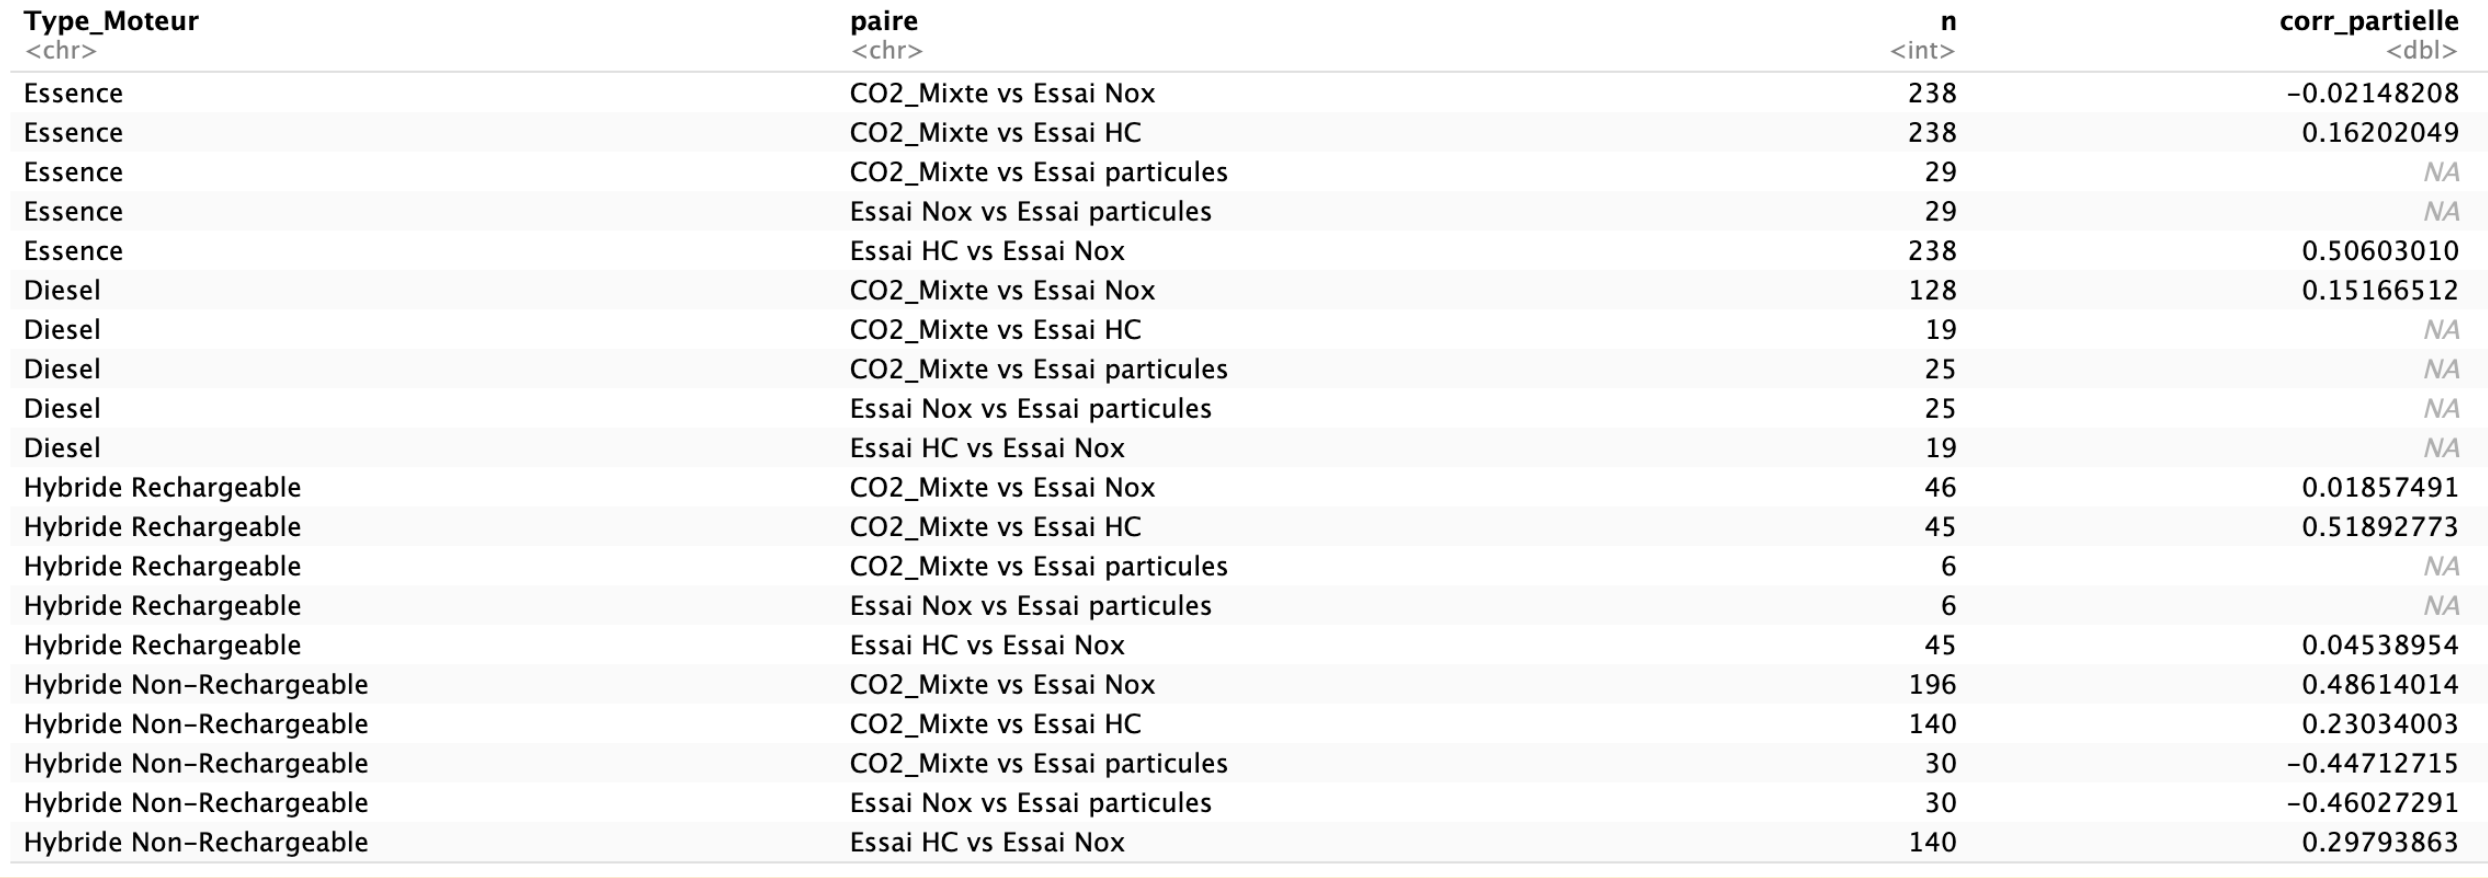
\includegraphics[width=\textwidth]{résultats/Corrélations_partielles.png}
    \caption{Matrice de corrélations partielles entre résidus d'émissions : synergies et compromis technologiques.}
    \label{fig:correlations_partielles}
\end{figure}

Le tableau présenté expose les corrélations partielles, c'est-à-dire les corrélations de Pearson calculées entre ces résidus. L'interprétation de ces coefficients est la suivante :

\vspace{0.6em}

\begin{itemize}
    \item Une corrélation positive (Synergie) : Un système techniquement optimisé pour abaisser le polluant A tend également à faire baisser le polluant B au-delà de ce que la physique du véhicule prédit.
\end{itemize}

\vspace{0.6em}

\begin{itemize}
    \item Une corrélation négative (Compromis / Trade-off) : Les efforts technologiques déployés pour minimiser le polluant A entraînent une dégradation structurelle des émissions du polluant B.
\end{itemize}

\subsubsection{Les Synergies : L'efficacité systémique de la post-combustion et de l'hybridation}

L'analyse du tableau révèle que, dans la majorité des configurations, l'ingénierie moderne parvient à créer des synergies vertueuses :

\vspace{0.5em}

\begin{itemize}
    \item Essence - HC vs NOx (0.506, n=238) : Cette forte corrélation positive est la signature mathématique de l'efficacité du pot catalytique "3 voies". Un système d'échappement bien dimensionné, chauffant rapidement et couplé à une gestion moteur précise (maintien du rapport stœchiométrique), parvient à optimiser simultanément l'oxydation des HC et la réduction des NOx.
\end{itemize}

\vspace{0.6em}

\begin{itemize}
    \item Hybride Non-Rechargeable - CO2 vs NOx (0.486, n=196) : Ce résultat confirme nos déductions issues de la SFA concernant la technologie "Full Hybrid". Les véhicules dotés d'une véritable hybridation utilisent le moteur électrique pour absorber les pics d'efforts. Le moteur thermique, fonctionnant dans des plages de charge optimales, voit son rendement s'améliorer (baisse du CO2) tout en évitant les surchauffes internes génératrices de la réaction de Zeldovich (baisse drastique des NOx). La synergie est ici totale.
\end{itemize}

\subsubsection{Le compromis fatal : Le mur technologique des Particules Fines (PM)}

Le résultat le plus critique de cette modélisation réside dans les corrélations négatives mises en évidence au sein du sous-échantillon des Hybrides Non-Rechargeables. Il convient de préciser d'emblée que le faible nombre d'observations disponibles pour les mesures de particules sur cette catégorie (n=30) limite la robustesse statistique de ce résultat et impose d'interpréter ces chiffres avec prudence. Néanmoins, ces corrélations illustrent un compromis d'ingénierie majeur et théoriquement très cohérent :

\vspace{0.6em}

\begin{itemize}
    \item CO2 vs Particules (-0.447) : Plus la technologie est optimisée pour minimiser le CO2, plus elle tend à générer des particules fines.
\end{itemize}

\vspace{0.6em}

\begin{itemize}
    \item NOx vs Particules (-0.460) : Plus le système est calibré pour éviter la formation de NOx, plus les émissions particulaires augmentent.
\end{itemize}

\vspace{0.6em}

Interprétation technologique : Ces corrélations négatives mettent en lumière le paradoxe de l'Injection Directe d'Essence (GDI), largement déployée sur les motorisations hybrides modernes pour maximiser le rendement thermique (baisse du CO2) et contrôler les températures de pointe (baisse des NOx). En injectant le carburant à très haute pression directement dans le cylindre (parfois en mode stratifié, au tout dernier moment), l'essence n'a pas toujours le temps de se vaporiser et de se mélanger de manière parfaitement homogène avec l'air. Des micro-gouttelettes brûlent incomplètement et se transforment en suie (particules fines). De plus, pour respecter les normes sur ces particules, les constructeurs doivent ajouter un Filtre à Particules Essence (GPF). Or, ce filtre crée une contre-pression à l'échappement qui pénalise légèrement le rendement du moteur, poussant ce dernier à consommer davantage et donc à ré-émettre du CO2.

\vspace{0.6em}

Notre modèle mathématique suggère ainsi que si l'automobile a résolu de nombreux défis historiques, la course à la réduction des gaz à effet de serre (CO2) s'est heurtée à un nouveau plafond de verre sanitaire : la recrudescence des particules fines à l'échappement.

\vspace{0.6em}

(Note méthodologique : Les valeurs NA figurant dans le tableau, particulièrement pour les motorisations Diesel concernant les HC et les particules, s'expliquent par des tailles d'échantillons exploitables trop faibles ou présentant une variance quasi nulle des résidus, ne permettant pas le calcul d'une corrélation statistiquement robuste et justifiant leur exclusion de cette analyse croisée).

\subsection{Palmarès d'efficience globale : L'optimisation technologique face à la réalité physique}

Pour synthétiser l'ensemble de nos modélisations par frontière stochastique, nous avons agrégé les scores SFA individuels (CO2, HC, NOx, HCNox) sous la forme d'une moyenne pondérée, créant ainsi une note globale d'efficience sur 100. Le tableau ci-dessus présente les véhicules les plus performants de notre échantillon selon ce critère multidimensionnel. L'analyse de ce palmarès met en lumière des dynamiques industrielles instructives et souligne l'intérêt d'une telle méthodologie pour contrôler les biais physiques.

\begin{figure}[H]
    \centering
    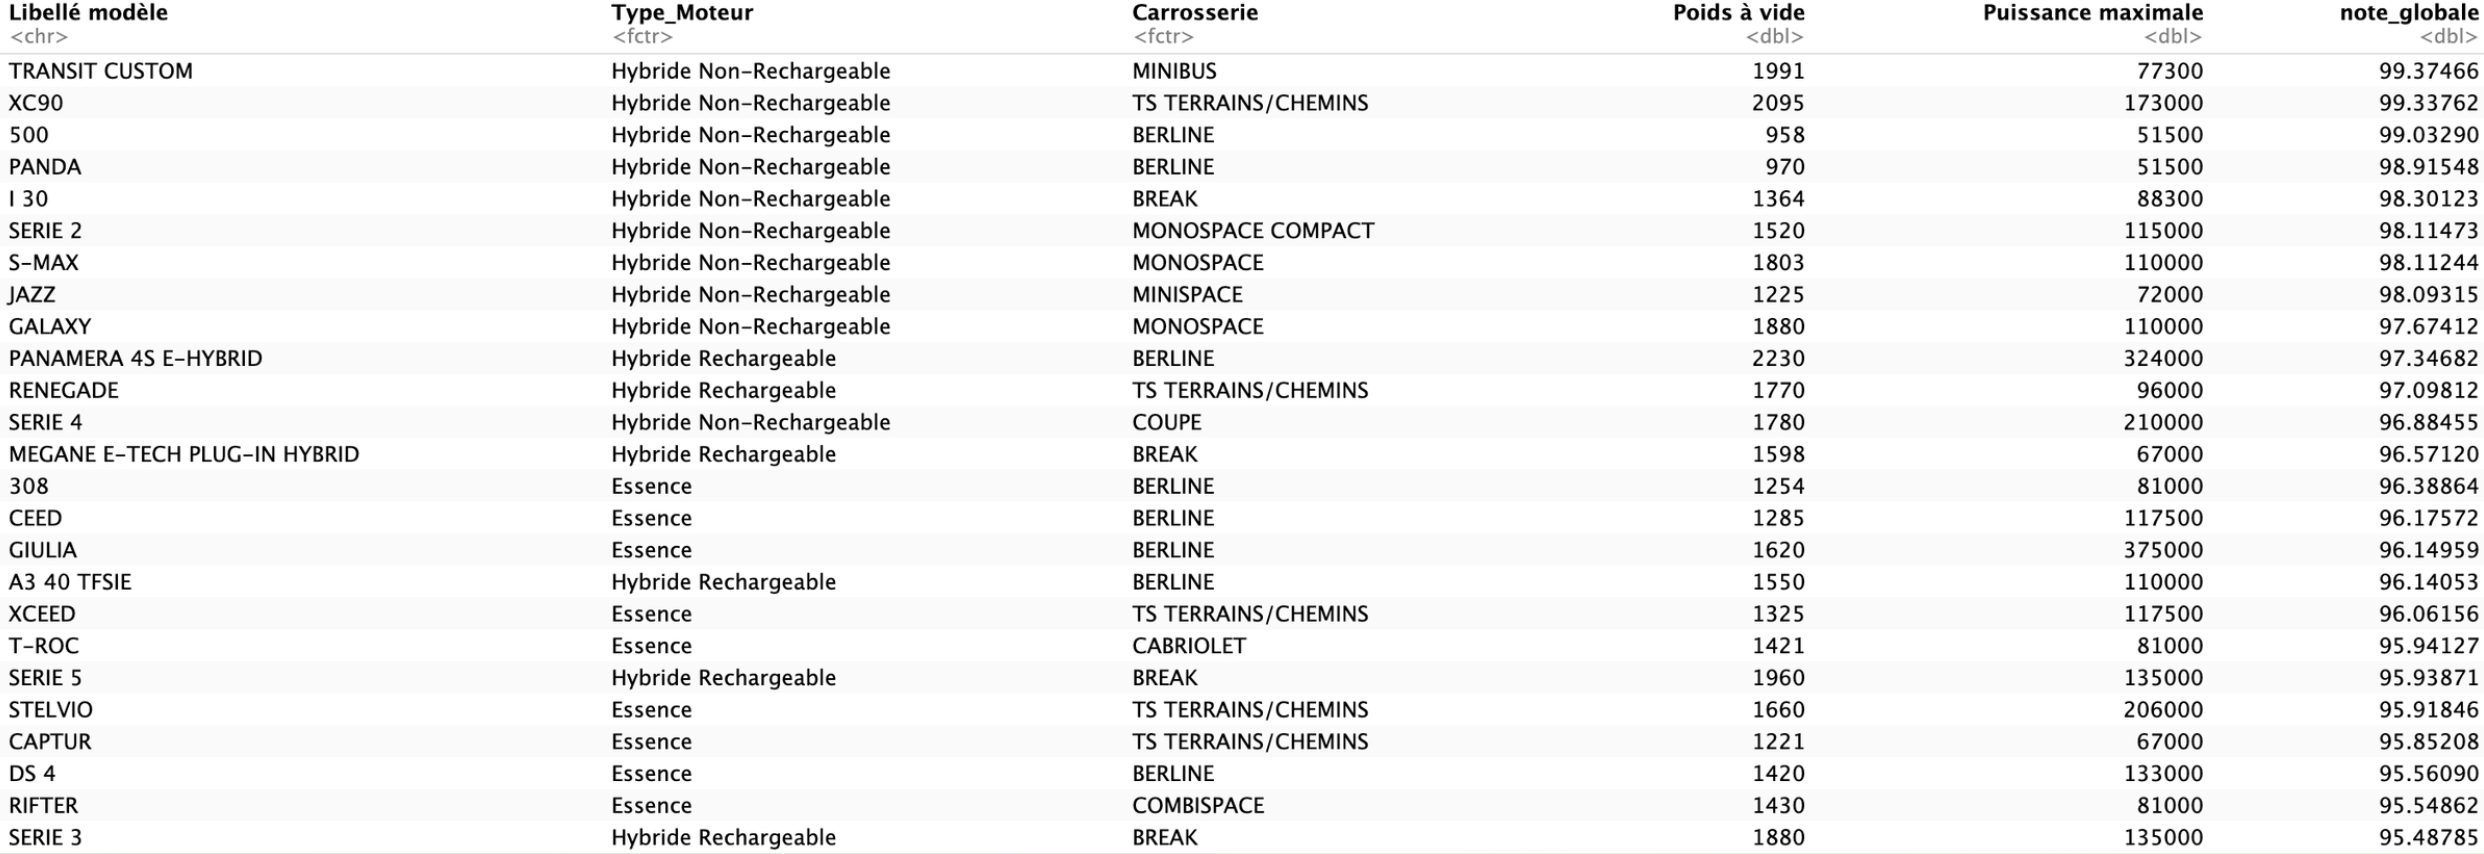
\includegraphics[width=\textwidth]{résultats/Classement_meilleurs_véhicules.png}
    \caption{Classement des véhicules les plus efficients selon l'indicateur global SFA multi-polluants.}
    \label{fig:classement_meilleurs}
\end{figure}

\vspace{0.6em}

Le premier enseignement de ce classement est la cohabitation de véhicules aux caractéristiques physiques diamétralement opposées. On retrouve en tête de classement des véhicules extrêmement lourds et peu aérodynamiques, tels que le Transit Custom (1991 kg, carrosserie Minibus) ou le Volvo XC90 (2095 kg, SUV), siégeant aux côtés de citadines très légères comme les Fiat 500 et Panda (moins de 1000 kg). Cette hétérogénéité tend à confirmer que notre modèle SFA parvient à neutraliser efficacement le biais lié au poids : il a réussi à "gommer" la pénalité inéluctable du poids. La note globale ne récompense pas le véhicule qui émet le moins de polluants dans l'absolu, mais celui dont l'ingénierie (groupe motopropulseur et post-traitement) est la plus proche de la perfection théorique compte tenu de son handicap physique de départ.

\vspace{0.6em}

L'écrasante domination de la catégorie "Hybride Non-Rechargeable" (qui monopolise les 9 premières places) est la confirmation empirique des synergies identifiées dans notre analyse des corrélations. Qu'il s'agisse de micro-hybridation optimisée sur des citadines légères (Fiat 500) ou de systèmes "Full Hybrid" très sophistiqués capables d'absorber les charges massives de véhicules lourds, l'assistance électrique non-rechargeable s'impose comme l'architecture la plus efficiente pour équilibrer la réduction du CO2 et la maîtrise des polluants locaux (NOx). Les véhicules thermiques purs (Essence), dépourvus de cette assistance, n'apparaissent que plus bas dans le classement, confirmant le plafond de verre technologique décrit précédemment.

\vspace{0.6em}

Il est crucial de conclure cette analyse empirique par une mise en garde fondamentale pour les politiques publiques. La présence d'un Porsche Panamera 4S E-Hybrid (2230 kg, 324 kW) ou d'un Volvo XC90 au sommet de ce palmarès d'efficience ne contredit en rien les lois de la thermodynamique exposées dans la première partie de notre rapport.

Le score exceptionnel (> 97/100) de ces véhicules très lourds signifie que leurs ingénieurs ont déployé des technologies de pointes (hybridation complexe, catalyseurs onéreux) pour minimiser la pollution générée par le déplacement de plus de 2 tonnes de métal. Cependant, l'efficience relative ne doit pas être confondue avec la sobriété absolue. En dépit de sa note parfaite traduisant une ingénierie de pointe, un SUV de 2 tonnes nécessitera toujours, en vertu des lois de l'énergie cinétique, significativement plus d'énergie et émettra in fine plus de rejets absolus (notamment des particules d'abrasion liées au freinage) qu'une citadine légère dotée d'une technologie plus basique.

Notre modèle SFA prouve ainsi que si l'industrie automobile excelle aujourd'hui dans l'optimisation technologique sous contrainte, cette prouesse technique atteint ses limites environnementales face à l'inflation continue de la masse des véhicules.

\subsection{Analyse des contre-performances : Les limites des architectures de compromis}

\begin{figure}[H]
    \centering
    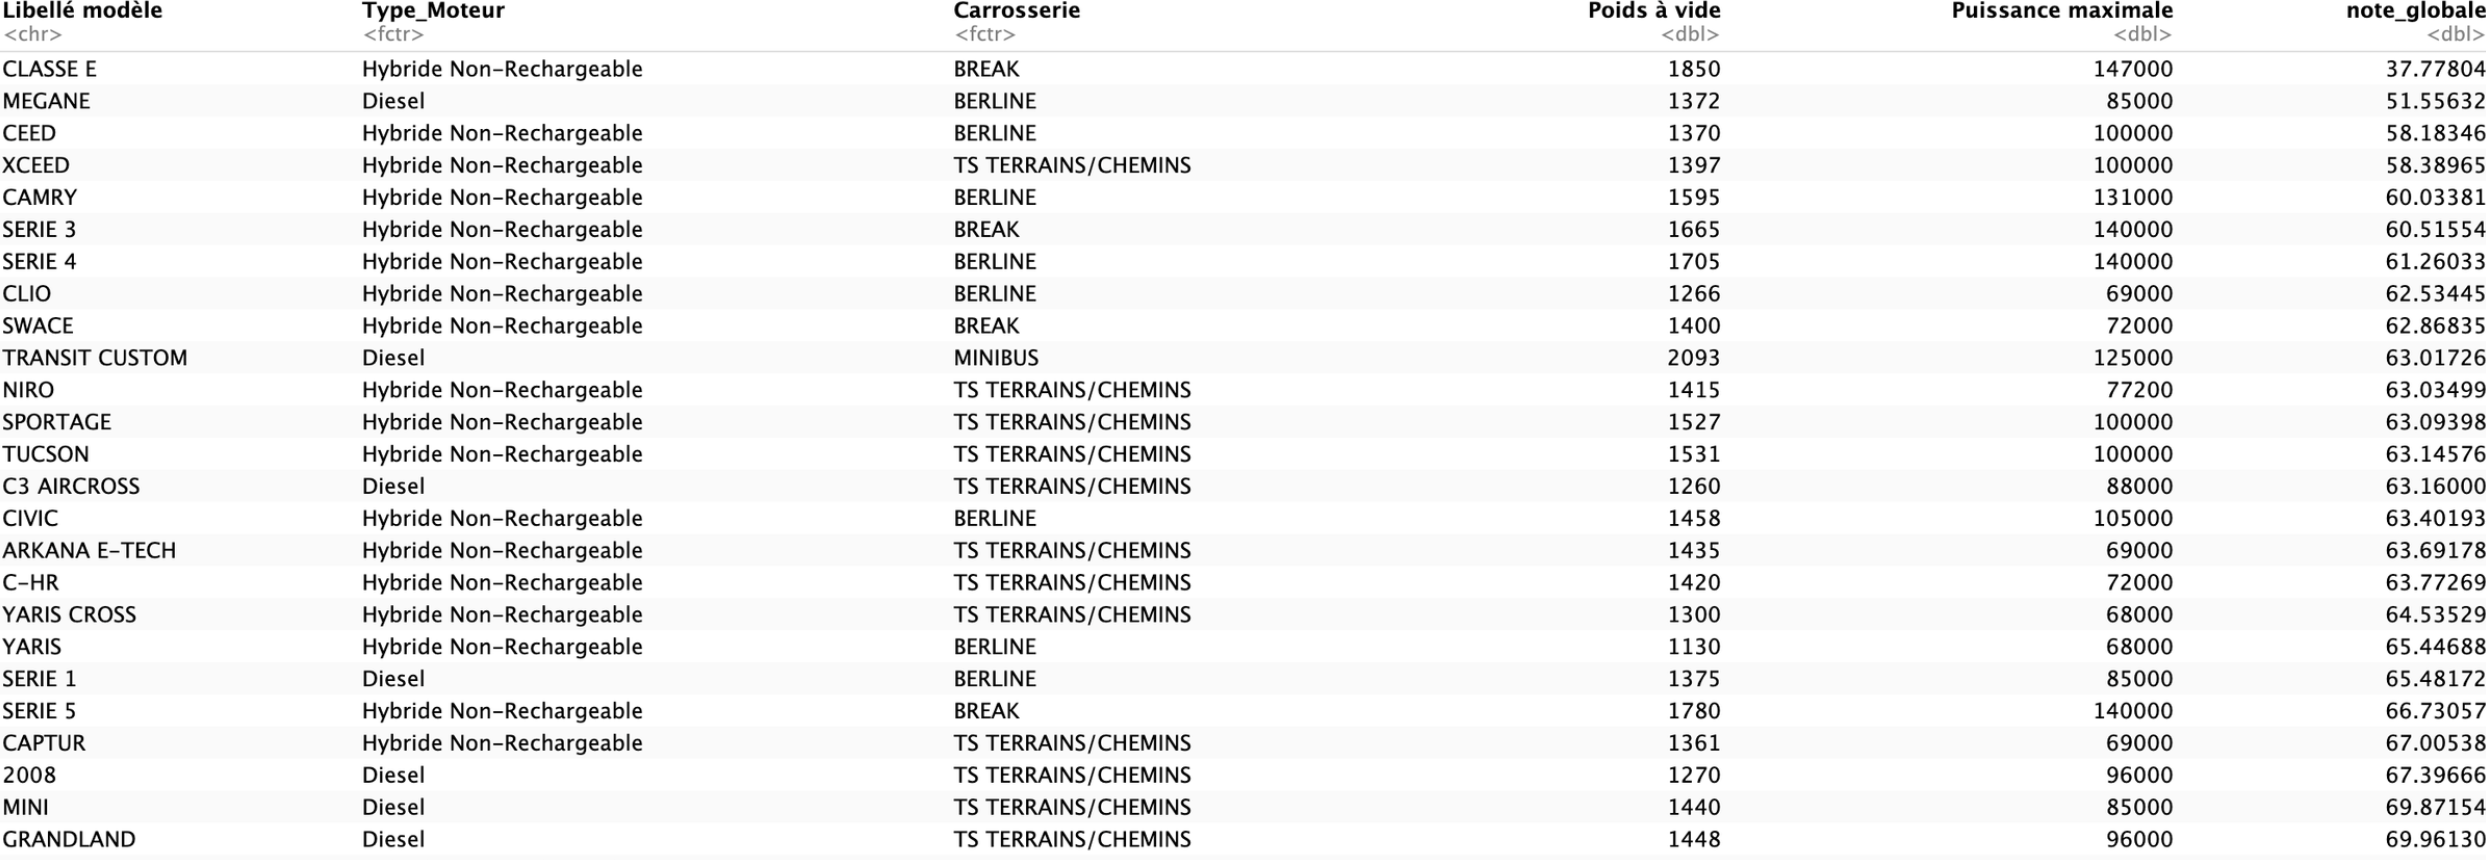
\includegraphics[width=\textwidth]{résultats/Classement_pires_véhicules.png}
    \caption{Classement des véhicules les moins efficients selon l'indicateur global SFA multi-polluants.}
    \label{fig:classement_pires}
\end{figure}

En miroir du palmarès précédent, l'observation des véhicules affichant les notes globales d'efficience les plus faibles (s'étalant de 37,7 à 69,9/100) apporte un éclairage complémentaire essentiel à notre étude. L'analyse de ce tableau corrobore nos précédentes modélisations sur les limites de certaines stratégies industrielles.

\vspace{0.6em}

Deux constats majeurs se dégagent de cet échantillon :

\vspace{0.6em}

La fracture confirmée de l'hybridation non-rechargeable Le résultat le plus frappant est la présence massive de la catégorie "Hybride Non-Rechargeable" dans le bas du classement, alors même qu'elle dominait le palmarès des véhicules les plus efficients. Cette apparente contradiction valide empiriquement la polarisation extrême identifiée lors de nos analyses SFA (notamment sur le CO2 et les NOx). Les véhicules présents dans ce tableau illustrent les limites de la micro-hybridation (Mild-Hybrid). Ces systèmes à bas coût, s'ils permettent d'optimiser les résultats bruts lors de l'homologation, s'avèrent structurellement inefficients pour compenser les contraintes physiques du véhicule en conditions réelles, se traduisant par des scores SFA relatifs très dégradés.

\vspace{0.6em}

Le plafond de verre du Diesel sans post-traitement optimal La seconde motorisation surreprésentée dans ces contre-performances est le Diesel. On y retrouve des véhicules variés (de la berline compacte comme la Mégane au véhicule utilitaire comme le Transit Custom). Leur présence dans le bas du tableau s'explique principalement par les résultats de l'efficacité SFA sur les oxydes d'azote (NOx). Comme souligné précédemment, un moteur Diesel qui ne bénéficie pas d'un système de post-traitement de pointe (de type SCR avec injection d'AdBlue), souvent pour des raisons de maîtrise des coûts sur certains segments, voit sa note globale s'effondrer, incapable de traiter efficacement les polluants liés à son fonctionnement en excès d'air.

\vspace{0.6em}

En synthèse, ce tableau des scores les plus faibles suggère que l'étiquette technologique (hybride ou diesel) ne suffit pas à garantir une véritable efficience thermodynamique et environnementale. Il met en exergue les "architectures de compromis", conçues davantage pour la conformité réglementaire que pour l'optimisation absolue du groupe motopropulseur.

\subsection{Classement des constructeurs : L'efficience technologique au prisme des stratégies de gamme}

\begin{figure}[H]
    \centering
    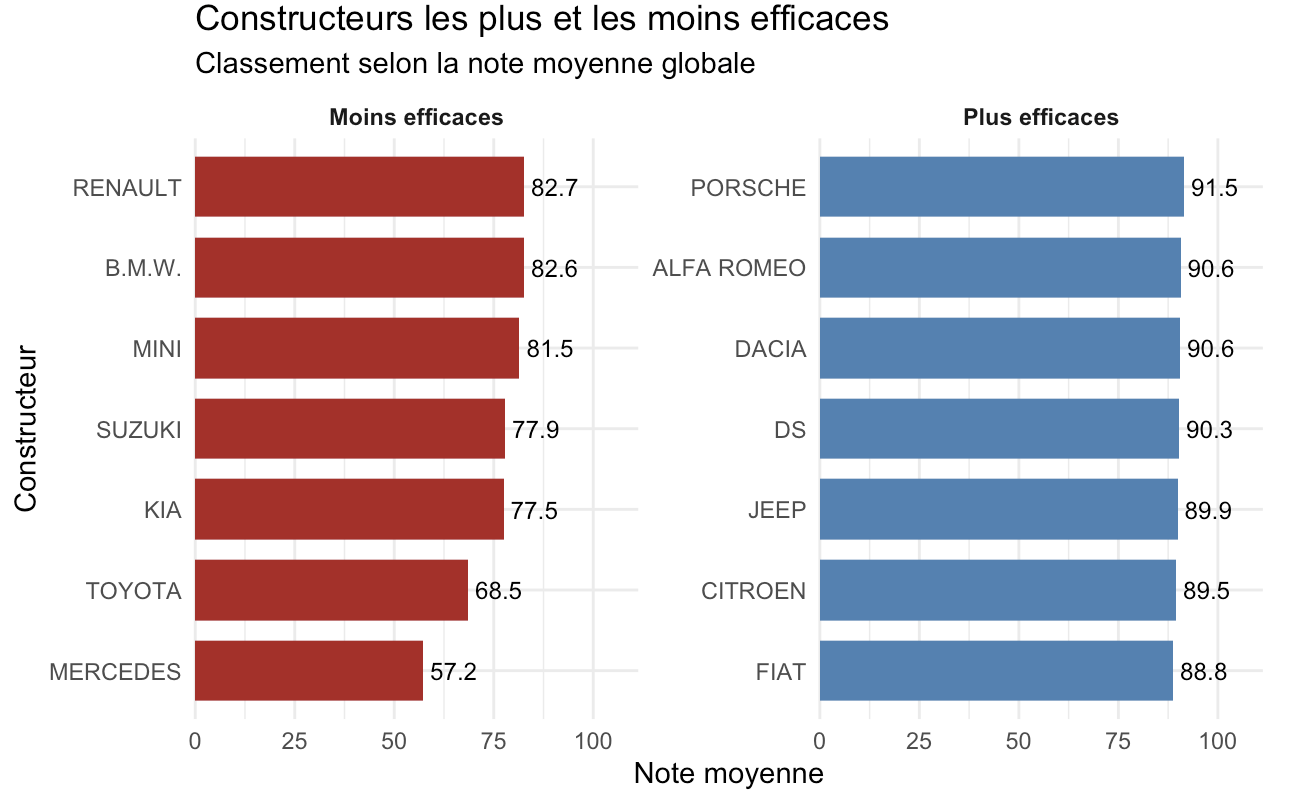
\includegraphics[width=\textwidth]{résultats/Classement_Constructeurs.png}
    \caption{Classement des constructeurs selon la moyenne des scores d'efficience globale.}
    \label{fig:classement_constructeurs}
\end{figure}

Pour achever cette analyse empirique, nous avons agrégé les notes globales d'efficience à l'échelle des constructeurs. Ce classement, basé sur la moyenne des scores SFA de l'ensemble des modèles proposés par chaque marque, offre une vision macroscopique des choix stratégiques industriels.

\vspace{0.6em}

Il est fondamental de rappeler ici la nature de cette note : elle ne mesure pas le volume absolu de pollution émis par la flotte d'un constructeur, mais évalue l'efficience relative de son ingénierie, une fois neutralisés les handicaps physiques (masse, puissance, aérodynamisme) de ses véhicules. Ce prisme d'analyse permet de déconstruire certains discours marketing et met en lumière trois dynamiques particulièrement instructives :

\vspace{0.6em}

\begin{itemize}
    \item Le paradoxe du segment Premium (Porsche vs Mercedes-Benz) : Le classement révèle une trajectoire diamétralement opposée entre des acteurs historiques du haut de gamme. D'un côté, Porsche domine le classement (91.5/100). Ce résultat tend à confirmer que sur des segments à très forte marge, le constructeur a la capacité financière d'intégrer des technologies de dépollution et d'hybridation sans compromis, parvenant à compenser de manière quasi optimale le handicap d'une masse très élevée. À l'inverse, Mercedes (57.2/100) et, dans une moindre mesure, BMW (82.6/100) affichent des contre-performances notables. Cela suggère que la démocratisation de l'hybridation sur l'ensemble de leur très large gamme s'est probablement appuyée sur des architectures dites "de transition" (comme la micro-hybridation MHEV). Si ces solutions permettent de passer les seuils d'homologation CO2, elles s'avèrent structurellement moins efficientes pour contrer la pénalité physique de leurs véhicules lourds sur un spectre multi-polluants.

    \vspace{0.5em}

    \item La performance inattendue des constructeurs généralistes et accessibles : La partie droite du graphique est largement occupée par des marques du groupe Stellantis (Fiat, Citroën, Jeep, DS, Alfa Romeo) ainsi que par Dacia (90.6/100). La présence de ces constructeurs, réputés pour des véhicules plus accessibles, démontre que l'efficience technologique n'est pas l'apanage du luxe. Ce résultat suggère que le recours à des motorisations thermiques matures, couplées à des architectures physiques potentiellement plus frugales à la base, permet d'atteindre un niveau d'optimisation très proche de la frontière théorique maximale définie par notre modèle.

    \vspace{0.5em}

    \item L'énigme Toyota : Les limites du compromis historique : L'apparition de Toyota (68.5/100) parmi les constructeurs les moins efficients de notre échantillon peut sembler contre-intuitive au regard de son statut de pionnier de l'hybridation. Toutefois, ce positionnement s'éclaire à la lumière de nos analyses précédentes sur les compromis (trade-offs). La stratégie historique de Toyota, massivement orientée vers la minimisation absolue de la consommation et du CO2 via des moteurs fonctionnant souvent en cycle d'Atkinson, pourrait présenter des vulnérabilités sur d'autres critères sanitaires (comme le traitement des NOx lors des transitoires de charge, ou les émissions de particules). Évaluée sous le prisme strict et multidimensionnel de la frontière stochastique, cette architecture technique de compromis affiche une efficience relative en deçà des attentes fixées par le modèle.
\end{itemize}

% ============================================================
\section{Conclusion Générale : Dépasser la Vision Tunnel pour une Régulation Holistique}
% ============================================================

L'objectif central de cette étude était de déconstruire l'approche unidimensionnelle des émissions automobiles, trop souvent cantonnée à la seule mesure du dioxyde de carbone (CO2). En croisant les principes de la thermodynamique avec une modélisation économétrique rigoureuse (OLS et SFA), notre analyse multi-polluants met en exergue les véritables dynamiques technologiques à l'œuvre au sein de l'industrie automobile, tout en révélant les profondes failles du cadre réglementaire et fiscal actuel.

\vspace{0.6em}

Le mur thermodynamique et l'illusion réglementaire : Notre démarche empirique, en neutralisant le biais de la masse et de l'aérodynamisme, a formellement démontré que la technologie des moteurs thermiques a atteint un plafond de maturité. Les variations d'émissions de CO2 ne relèvent plus de l'efficience de l'ingénierie, mais sont une traduction directe et incompressible de l'inflation de la masse des véhicules. Par ailleurs, l'étude souligne les limites béantes des procédures d'homologation actuelles (cycle WLTP). Ces tests ont engendré des "architectures de conformité" : des véhicules hybrides rechargeables (PHEV) et micro-hybrides (MHEV) optimisés pour briller en laboratoire, mais dont notre Analyse de Frontière Stochastique a révélé la profonde inefficacité structurelle en conditions réelles, particulièrement face au défi sanitaire des oxydes d'azote (NOx).

\vspace{0.6em}

Le grand angle mort : Les Particules Fines (PM) et la rareté des données. L'une des limites majeures de notre propre analyse reflète paradoxalement la faille la plus critique du système d'homologation européen : le manque flagrant de données sur les particules fines. Alors que ces particules (PM2.5 et PM10) constituent un enjeu de santé publique majeur (infiltrant le système sanguin et neurologique), elles sont les grandes absentes des bases de données de certification pour une écrasante majorité de motorisations à essence et hybrides. Le faible échantillon exploitable dans notre étude (n=30 pour les hybrides) nous a tout de même permis d'identifier mathématiquement un compromis (trade-off) fatal : les technologies d'injection directe (GDI), déployées massivement pour faire baisser la consommation et le CO2, génèrent mécaniquement une hausse des rejets de particules fines. L'incapacité actuelle des procédures de test à imposer une mesure systématique et rigoureuse de ces particules occulte une part dramatique de la pollution réelle du parc automobile moderne.

\vspace{0.6em}

L'obsolescence du système de Bonus-Malus : Ces conclusions empiriques invitent à une refonte urgente des politiques publiques, et tout particulièrement du système de bonus-malus écologique français. Dans sa configuration actuelle, cette fiscalité est l'incarnation même de la "vision tunnel" dénoncée tout au long de ce rapport. En se focalisant exclusivement sur un seuil de CO2 et, plus récemment, sur un malus au poids (souvent contourné par des exemptions pour les véhicules hybrides), l'État subventionne aveuglément des technologies sans tenir compte de leur impact sanitaire global. Un SUV lourd hybride rechargeable peut ainsi échapper au malus au poids et bénéficier d'une fiscalité avantageuse sur le CO2, alors même que notre étude démontre que son efficience sur la dépollution locale (NOx et HC) peut être désastreuse dès que sa batterie est vide.

\subsection{Perspectives}

La régulation automobile ne peut plus faire l'économie d'une approche holistique. Pour que l'industrie réponde conjointement à l'urgence climatique (CO2) et sanitaire (NOx, PM), les politiques fiscales et réglementaires doivent impérativement intégrer un index multi-polluants. Tant que les émissions d'oxydes d'azote et de particules fines ne pèseront pas sur le prix d'achat des véhicules au même titre que le carbone, et tant que la masse continuera d'être compensée par des artifices d'homologation, l'efficience technologique restera subordonnée à une logique de contournement plutôt qu'à une véritable sobriété environnementale.
